% !TEX encoding = UTF-8
% !TEX TS-program = pdflatex
% !TEX root = ../arsclassica.tex
% !TEX spellcheck = it-IT

%************************************************
\chapter{Esperimenti numerici}\label{cap:esperimenti}
%************************************************
Lo scopo finale di questo capitolo è presentare i risultati ottenuti dalla sperimentazione del processo di \emph{classificazione supervisionata\index{classificazione!profili di traffico}} utilizzando diversi modelli di classificatore \acs{CTBN} (\acs{CTBNC}) (riguardo tali argomenti si rimanda ai~\vref{cap:ctbnc,cap:structurallearning}).

Tuttavia, prima di illustrare e comparare i succitati risultati, si presentano i modelli \acs{TSIS} da cui sono stati generati i dataset oggetto della sperimentazione. La generazione di dataset inerenti il traffico automobilistico è stata effettuata, come detto, tramite un software commerciale apposito, \acs{TSIS}, e una \acl{RTE}, \acsfont{Sensors} \acs{DLL}, sviluppata a tale fine. Per maggiori dettagli riguardanti questi strumenti si rimanda al \vref{cap:tsis-sensors}.

Perciò, questo capitolo è così articolato: una sezione per ognuno dei $2$ dataset generati, e una sezione relativa alla succitata sperimentazione. Le sezioni relative ai dataset sono suddivise in due sottosezioni: la prima finalizzata alla descrizione del modello \acs{TSIS} da cui è stato generato il dataset successivamente sottoposto a sperimentazione e la seconda finalizzata alla presentazione delle varie configurazioni del dataset generato.

Al fine di valutare l'accuratezza dei metodi predittivi sviluppati, la sperimentazione è stata eseguita utilizzando la tecnica chiamata \emph{\keyword{cross-validazione}}. Tale metodologia di validazione è infatti pensata per accertare la capacità di generalizzazione di un modello statistico di tipo predittivo su un insieme di dati non conosciuto. Nello specifico, le sperimentazioni dei metodi predittivi valutati sono state condotte tramite una \emph{$k$-fold\index{cross-validazione!$k$-fold}} \emph{\keyword{cross-validazione}} con $k=10$\index{$k$-fold|see{cross-validazione}}.

\section{\Ds{1}}\label{sec:dataset-1}
Lo scopo di questa sezione è presentare le varie configurazioni del \ds{1} create.

\subsection{Modello TSIS}\label{subsec:tsis-simple-model}
Al fine di introdurre il \ds{1}\index{dataset} è necessario presentare la rete stradale \acs{TSIS} e il relativo modello di simulazione\index{\acsfont{CORSIM}!modello di simulazione} \acs{CORSIM} da cui esso è stato generato.

La~\vref{fig:tsis-model-simple} mostra la rete stradale che compone il modello \acs{TSIS} oggetto di questa sottosezione.
\begin{figure}[H]
  	\centering
  	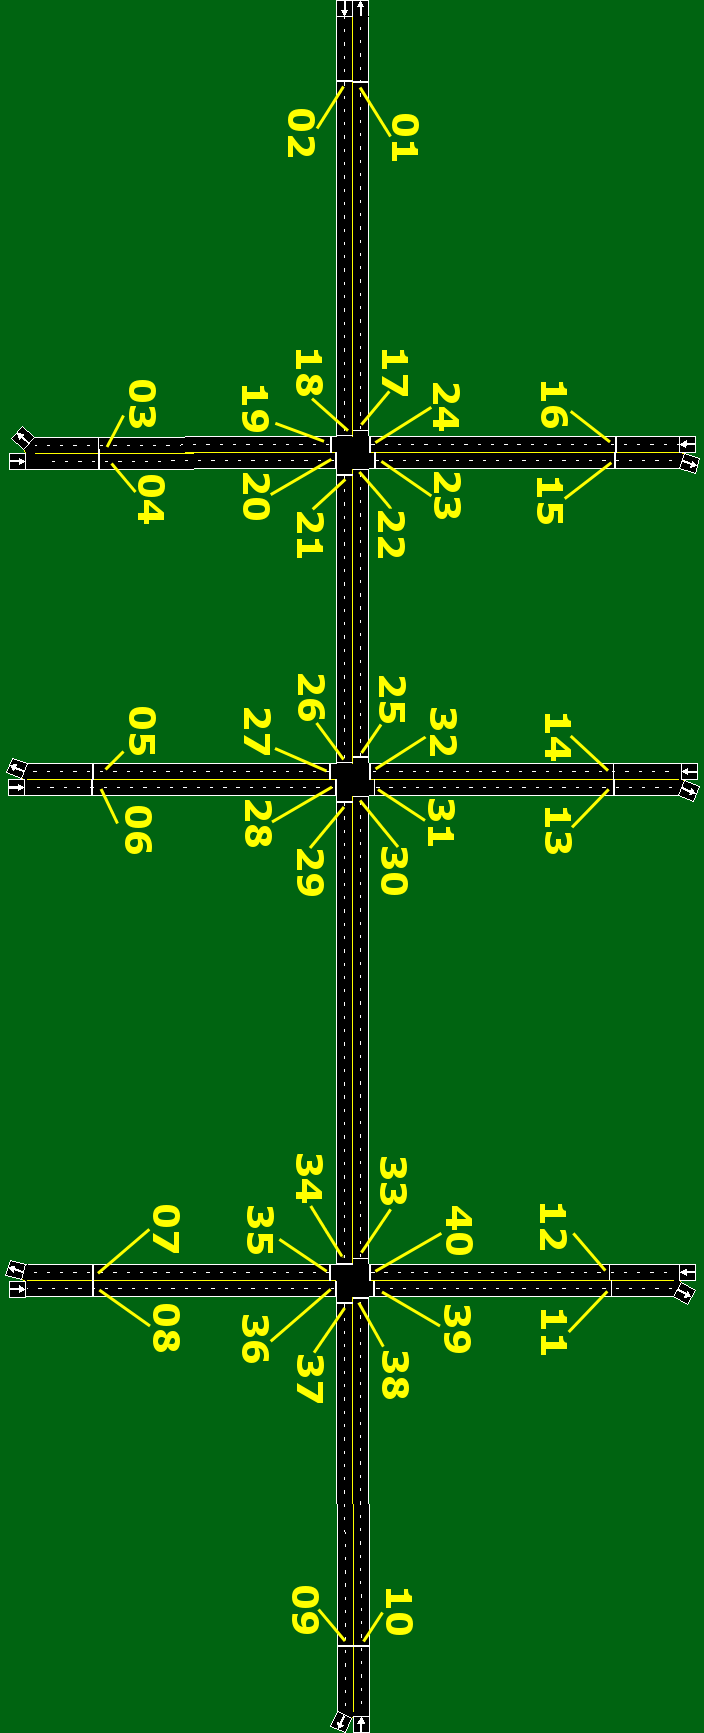
\includegraphics[max size={0.9\textwidth}{0.9\textheight}]{tsis-model-simple}%
  	\caption[Rete stradale relativa al \ds{1}]{Visualizzazione del file \acs{TNO} rappresentante la rete stradale da cui viene generato il \ds{1}. I sensori sono etichettati tramite degli indici numerici di colore giallo mentre i nodi sono etichettati tramite degli indici numerici di colore bianco.}
	\label{fig:tsis-model-simple}
\end{figure}
Tale figura evidenzia:
\begin{itemize}
	\item la disposizione dei sensori (indicati tramite degli indici numerici di colore giallo) utilizzati per il monitoraggio del passaggio dei veicoli
	\item le strade, tutte composte da $2$ corsie, e i nodi (indicati tramite degli indici numerici di colore bianco) da cui è composta la rete stradale
	\item i sensi di marcia delle corsie
\end{itemize}
Di seguito si riportano le ulteriori caratteristiche di tale rete stradale:
\begin{itemize}
	\item la larghezza delle corsie è \num{3.65} \si{\metre}
	\item la lunghezza della strada principale (\ie{} da nodo $01$ a nodo $05$) è \num{780} \si{\metre} mentre la lunghezza delle strade ad essa perpendicolari è pari a \num{300} \si{\metre}
	\item la dimensione dei sensori è \num{0.30} \si{\metre}, da cui consegue che la dimensione della zona sensibile (in tutte le direzioni) è \num{2.13} \si{\metre}
	\item la distanza dei sensori dal nodo più vicino è \num{6.5} \si{\metre}
\end{itemize}

Le intersezioni principali della rete stradale (\ie{} nodi con indici $02$, $03$ e $04$ nella~\vref{fig:tsis-model-simple}) sono controllate da semafori il cui ciclio di controllo dura $100$ secondi. La~\vref{fig:tsis-model-simple-controls} illustra la configurazione del piano semaforico per ogni intersezione controllata durante tutto il tempo di simulazione.
\begin{figure}[H]
	\centering
	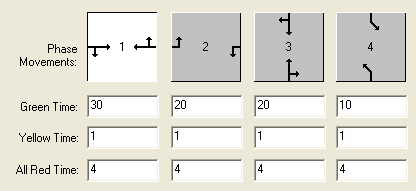
\includegraphics[width=0.75\columnwidth,keepaspectratio]{tsis-model-simple-controller}
	\caption[Piano semaforico relativo al \ds{1}]{Piano semaforico predefinito delle intersezioni $02$, $03$ e $04$ della rete stradale \acs{TSIS} relativa al \ds{1}.}
	\label{fig:tsis-model-simple-controls}
\end{figure}

Come anticipato, ogni strada che compone la rete stradale contiene, nei pressi dei nodi (sia che essi siano delle intersezioni, sia che essi siano dei nodi di ingresso o di transito), dei sensori finalizzati al rilevamento e tracciamento del passaggio dei veicoli: essi sono indicati nella~\vref{fig:tsis-model-simple} da indici numerici di colore giallo. La~\vref{tab:ds-1-sensors-indices} elenca il nome reale di tali sensori, utilizzato per la generazione del relativo dataset (a tal riguardo, un esempio di dataset è stata riportato nella~\autoref{subsec:sensors-dll-output}~\vpageref{subsec:sensors-dll-output}).
\begin{table}[htbp]%
	\centering%
	\begin{tabular}{+l^l}
	\toprule\rowstyle{\bfseries}%
	\# & Sensore  \\\otoprule
	$01$& D$212$\\
	$02$& D$121$\\
	$03$& D$272$\\
	$04$& D$721$\\
	$05$& D$392$\\
	$06$& D$931$\\
	$07$& D$4412$\\
	$08$& D$1141$\\
	$09$& D$452$\\
	$10$& D$541$\\\bottomrule
	\end{tabular}
	\hspace{-0.6em}
	\begin{tabular}{+l^l}
	\toprule\rowstyle{\bfseries}%
	\# & Sensore  \\\otoprule
	$11$& D$4102$\\
	$12$& D$1041$\\
	$13$& D$382$\\
	$14$& D$831$\\
	$15$& D$262$\\
	$16$& D$621$\\
	$17$& D$211$\\
	$18$& D$122$\\
	$19$& D$271$\\
	$20$& D$722$\\\bottomrule
	\end{tabular}
	\hspace{-0.6em}
	\begin{tabular}{+l^l}
	\toprule\rowstyle{\bfseries}%
	\# & Sensore  \\\otoprule
	$21$& D$231$\\
	$22$& D$322$\\
	$23$& D$261$\\
	$24$& D$622$\\
	$25$& D$321$\\
	$26$& D$232$\\
	$27$& D$391$\\
	$28$& D$932$\\
	$29$& D$341$\\
	$30$& D$432$\\\bottomrule
	\end{tabular}
	\hspace{-0.6em}
	\begin{tabular}{+l^l}
	\toprule\rowstyle{\bfseries}%
	\# & Sensore  \\\otoprule
	$31$& D$381$\\
	$32$& D$832$\\
	$33$& D$431$\\
	$34$& D$342$\\
	$35$& D$4111$\\
	$36$& D$1142$\\
	$37$& D$451$\\
	$38$& D$542$\\
	$39$& D$4101$\\
	$40$& D$1042$\\\bottomrule
	\end{tabular}
	\caption[Sensori del \ds{1}]{Corrispondenza fra gli identificatori dei sensori del \ds{1} e l'indice con cui essi sono indicati nella~\autoref{fig:tsis-model-simple}.}
	\label{tab:ds-1-sensors-indices}
\end{table}

Il modello di simulazione \acs{CORSIM} creato per questa rete stradale prevede un tempo di simulazione totale pari a $24$ ore, suddiviso in $16$ \emph{time period\index{dataset!time period}}, ognuno dei quali composto da \emph{time interval\index{dataset!time interval}} della durata di $1$ secondo: la~\vref{tab:ds-1-tp-labels} illustra la durata (in ore) di ognuno di essi e introduce la corrispondenza fra essi e la fase della giornata, rappresentata come la variabile classe nel relativo dataset.
\begin{table}[htbp]%
	\centering%
	\begin{tabular}{+l^l^l^l}
	\toprule\rowstyle{\bfseries}%
	Fascia oraria  		   & Time Period  	& Fase          & Classe  \\\otoprule
	$07$:$00$ - $08$:$00$  & $1$            & mattino       & $1$     \\
	$08$:$00$ - $09$:$00$  & $2$            & mattino       & $1$     \\
	$09$:$00$ - $10$:$00$  & $3$            & mattino       & $1$     \\
	$10$:$00$ - $12$:$00$  & $4$            & giorno        & $2$     \\
	$12$:$00$ - $14$:$00$  & $5$            & giorno        & $2$     \\
	$14$:$00$ - $16$:$00$  & $6$            & giorno        & $2$     \\
	$16$:$00$ - $17$:$00$  & $7$            & giorno        & $2$     \\
	$17$:$00$ - $18$:$00$  & $8$            & pomeriggio    & $3$     \\
	$18$:$00$ - $19$:$00$  & $9$            & pomeriggio    & $3$     \\
	$19$:$00$ - $20$:$00$  & $10$           & pomeriggio    & $3$     \\
	$20$:$00$ - $22$:$00$  & $11$           & sera          & $4$     \\
	$22$:$00$ - $24$:$00$  & $12$           & sera          & $4$     \\
	$00$:$00$ - $02$:$00$  & $13$           & notte         & $5$     \\
	$02$:$00$ - $04$:$00$  & $14$           & notte         & $5$     \\
	$04$:$00$ - $05$:$00$  & $11$           & notte         & $5$     \\
	$05$:$00$ - $07$:$00$  & $16$           & alba          & $6$     \\\bottomrule
	\end{tabular}
	\caption[Periodi temporali relativi al \ds{1}]{Caratterizzazione dei periodi temporali (\ie{} \emph{time period\index{dataset!time period}}) del modello \acs{TSIS} relativo al \ds{1}.}
	\label{tab:ds-1-tp-labels}
\end{table}

Ogni fase della giornata (\ie{} classe) è caratterizzata da un andamento diverso del traffico:
\begin{itemize}
	\item al mattino traffico intenso su tutta la rete stradale e code in direzione del nodo $05$
	\item durante il giorno traffico moderato su tutta la rete e code residue verso il nodo $05$ nella prima parte di tale fase
	\item nel pomeriggio traffico intenso su tutta la rete stradale e code in direzione del nodo $01$
	\item durante la sera traffico moderato su tutta la rete stradale e code residue verso il nodo $01$ nella prima parte di tale fase
	\item durante la notte pochi veicoli in tutte le direzioni
	\item all'alba aumento dei veicoli diretti verso il nodo $05$
\end{itemize}

L'andamento del traffico è modellato in \acs{CORSIM} variando i flussi di ingresso dei veicoli e le percentuali di svolta nelle varie intersezioni al variare dei periodi temporali o, in generale, delle fasi di simulazione previste. La~\vref{tab:ds-1-input-vehicles} illustra i flussi di ingresso nella rete stradale, espressi come numero di veicoli orari (\ie{} \si{vph}), per ogni fase della simulazione. Si osservi che l'immissione di veicoli sulla rete stradale avviene seguendo una distribuzione di probabilità di Erlang con parametro \emph{shape} pari a $2$.
\begin{table}[H]
	\centering
	\begin{tabular}{+l^c^c^c}
	\toprule\rowstyle{\bfseries}%
	Fase 		& $01 \rightarrow 05$ & $05 \rightarrow 01$ & Strade secondarie	\\
				& \si{vph}			  & \si{vph}			& \si{vph}			\\\otoprule
	mattino		& $600$ 			  & $200$			  	& $100$				\\
	giorno 		& $300$				  & $300$			    & $50$				\\
	pomeriggio	& $200$				  & $600$			    & $100$				\\
	sera 		& $100$				  & $200$			    & $50$				\\
	notte 		& $50$				  & $50$			    & $25$				\\
	alba		& $200$				  & $100$			    & $50$				\\\bottomrule
	\end{tabular}
	\caption[Flussi di ingresso relativi al \ds{1}]{Numero di veicoli orari immessi nella rete stradale del dataset \ds{1} al variare della fase di simulazione.}
	\label{tab:ds-1-input-vehicles}
\end{table}

La~\vref{tab:ds-1-turning-movs} illustra le percentuali di svolta al variare della fase di simulazione. L'intestazione di tale tabella indica i nodi di provenienza dei veicoli, il senso di marcia e le direzioni previste dall'intersezione che segue il nodo di partenza. Le celle invece indicano la distribuzione delle svolte effettuate dai veicoli nelle intersezioni.

Si consideri, ad esempio, la prima cella della~\autoref{tab:ds-1-turning-movs}: l'$80$\% dei veicoli provenienti dai nodi $01$, $02$ e $03$, giunti alle intersezioni che seguono tali nodi (\ie{} nodi $02$, $03$ e $04$, rispettivamente; si veda a tal riguardo la~\vref{fig:tsis-model-simple}), proseguono senza svoltare; il $10$\% dei veicoli provenienti dai nodi $01$, $02$ e $03$, invece, svolterà verso destra; idem verso sinistra.
\begin{table}[htbp]
	\centering\footnotesize
	\begin{tabular}{+l^c^c^c^c^c^c^c^c^c^c^c^c}
	\toprule\rowstyle{\bfseries}%
	Nodi & \multicolumn{3}{c}{$01$ - $02$ - $03$} & \multicolumn{3}{c}{$03$ - $04$ - $05$} & \multicolumn{3}{c}{$06$ - $08$ - $10$} & \multicolumn{3}{c}{$07$ - $09$ - $11$} \\
	& & $\longrightarrow$ &
	& & $\longleftarrow$  &
	& & $\longrightarrow$ &
	& & $\longleftarrow$  &\\
	& $\hookleftarrow$ & $\hookrightarrow$ & $\downarrow$
	& $\hookleftarrow$ & $\hookrightarrow$ & $\downarrow$
	& $\searrow$ & $\hookrightarrow$ & $\downarrow$
	& $\nwarrow$ & $\hookrightarrow$ & $\downarrow$\\
	& & \% &
	& & \% &
	& & \% &
	& & \% &\\\otoprule
	mattino 	& $10$ & $10$ & $80$ & $20$ & $20$ & $60$ & $80$ & $10$ & $10$ & $10$ & $80$ & $10$ \\
	giorno  	& $20$ & $20$ & $60$ & $20$ & $20$ & $60$ & $60$ & $20$ & $20$ & $20$ & $60$ & $20$ \\
	pomeriggio 	& $20$ & $20$ & $60$ & $10$ & $10$ & $80$ & $10$ & $80$ & $10$ & $80$ & $10$ & $10$ \\
	sera 		& $40$ & $40$ & $20$ & $10$ & $10$ & $80$ & $30$ & $40$ & $30$ & $40$ & $30$ & $30$ \\
	notte 		& $33$ & $33$ & $33$ & $33$ & $33$ & $33$ & $33$ & $33$ & $33$ & $33$ & $33$ & $33$ \\
	alba 		& $10$ & $10$ & $80$ & $40$ & $40$ & $20$ & $40$ & $30$ & $30$ & $30$ & $40$ & $30$ \\\bottomrule
	\end{tabular}
	\caption[Percentuali di svolta relative al \ds{1}]{Percentuali di svolta dei veicoli per ogni intersezione della rete stradale del \ds{1}, al variare della fase di simulazione.}
	\label{tab:ds-1-turning-movs}
\end{table}

\newpage
\subsection{Configurazioni del dataset}
Come detto nella~\autoref{subsec:sensors-dll}~\vpageref{subsec:sensors-dll}, eseguendo il modello di simulazione \acs{CORSIM} descritto in questa sezione con \acsfont{Sensors} \acs{DLL} si ottiene un file di output (si veda il listato d'esempio \ref{lst:sensors-out-format} \vpageref{lst:sensors-out-format}) che, adeguatamente processato, compone un \keyword{dataset} sottoponibile agli algoritmi di apprendimento e classificazione\index{classificazione!profili di traffico} presentati nei capitoli~\ref{cap:ctbnc} e \ref{cap:structurallearning}.

Di seguito si descrivono le caratteristiche di tale dataset comuni a tutte le sue varianti generate:
\begin{itemize}
	\item tempo totale pari a $86400$ secondi (\ie{} $24$ ore)
	\item la colonna \lstinline[]|tp| è stata rimossa e sostituita con la colonna \lstinline[]|class| in base alla corrispondenza riportata nella \vref{tab:ds-1-tp-labels}
	\item l'intestazione di ogni elemento è: \\ \lstinline[]|time, class, D122, D121, D341, D342, D722, D721, D1142, D1141, D231, D232, D541, D542, D4112, D4111, D431, |\\\lstinline[]|D432, D4101, D4102, D451, D452, D832, D831, D261, D262, D321, D322, D392, D391, D211, D212, D272, D271, D1042, |\\\lstinline[]|D1041, D622, D621, D932, D931, D381, D382|.
	\item ogni elemento del dataset (\ie{} file) è stato ottimizzato, cioè sottoposto all'eliminazione delle righe in cui non si verifica alcuna transizione di stato dei sensori
\end{itemize}

Per il dataset in questione si sono create due sue differenti varianti operando differenti divisioni temporali del file sorgente:
\begin{enumerate}
	\item suddivisione in $864$ elementi, ognuno dei quali include al più $100$ secondi di traiettoria\index{traiettoria} di ogni sensore della succitata rete stradale
	\item suddivisione in $288$ elementi, ognuno dei quali include al più $5$ minuti di traiettorie di ogni sensore della succitata rete stradale.
\end{enumerate}
Tali configurazioni sono chiamate, rispettivamente, \ds{1\text{.}100} e \ds{1\text{.}300}.

\cleardoublepage
\section{\Ds{2}}\label{sec:dataset-2}
Questa sezione presenta il \ds{2}. A tale scopo, nella sottosezione che segue, si descrive la rete stradale \acs{TSIS} e il relativo modello di simulazione \acs{CORSIM} da cui tale \keyword{dataset} è stato generato.

\subsection{Modello TSIS}\label{subsec:tsis-monza-model}
Il modello \acs{TSIS}\index{\acsfont{CORSIM}!modello di simulazione} in questione, a differenza di quello presentato nella \autoref{subsec:tsis-simple-model}, riproduce una rete stradale reale. Nello specifico esso riproduce la rete stradale circostante \emph{Viale Cesare Battisti} ($20900$ \emph{Monza, MB - Italia}). Disponendo di una serie di informazioni reali, tra cui i dati dei sensori posti su tale rete stradale, si sono potute inferire le caratteristiche della circolazione dei veicoli (\eg{} flusso di veicoli in ingresso) e quindi riprodurre fedelmente l'andamento del traffico durante tutti i giorni della settimana tramite degli adeguati modelli di simulazione \acs{CORSIM}. Nello specifico si sono realizzati $3$ modelli \acs{CORSIM}: essi rappresentano la stessa rete stradale ma diversi modelli di traffico, uno per i giorni lavorativi (dal lunedì al venerdì), uno per il sabato e uno per la domenica.

La~\vref{fig:tsis-model-monza-nodes} illustra la rete stradale oggetto di studio, evidenziando e identificando i nodi e i collegamenti stradali utilizzati per la sua riproduzione in \acs{TSIS}.
\begin{figure}
  \centering
  \captionsetup[subfigure]{labelformat=empty}
  \subfloat[][]{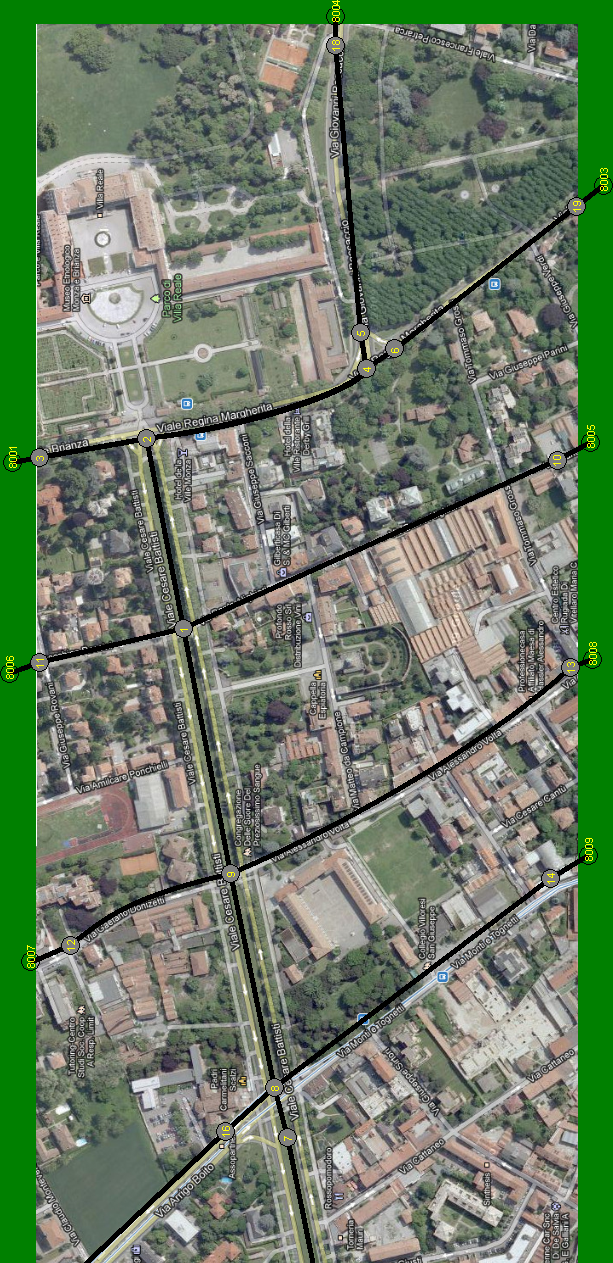
\includegraphics[width=0.99\columnwidth]{tsis-model-monza-gmap-dx}}%
  \phantomcaption
  \label{fig:tsis-model-monza-nodes}
\end{figure}
\begin{figure}[ht]
  \centering
  \captionsetup{type=figure}
  \captionsetup[subfigure]{labelformat=empty}
  \subfloat[][]{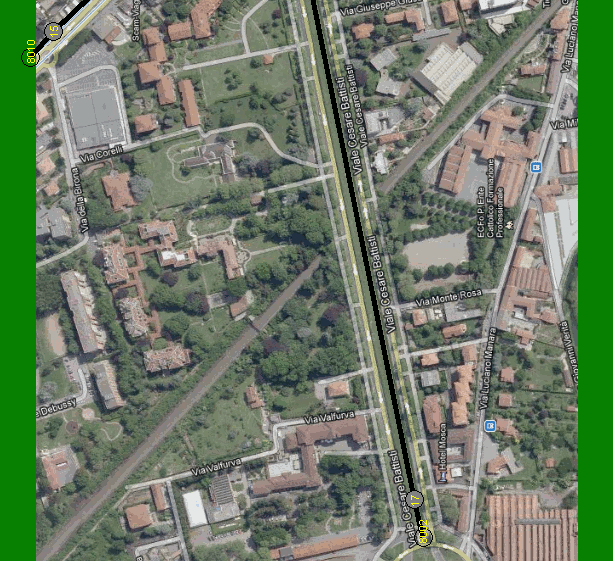
\includegraphics[width=0.99\columnwidth]{tsis-model-monza-gmap-sx}}%
  \caption[Intersezioni della rete stradale del \ds{2}]{Visualizzazione del file \acs{TNO} rappresentante le intersezioni della rete stradale da cui viene generato il \ds{2}.}
\end{figure}

La~\vref{tab:ds-2-nodes} illustra invece la correlazione tra gli indici dei nodi \acs{CORSIM} e ciò che essi rappresentano nel modello in questione.
\begin{table}[htbp]%
	\centering%
	\begin{tabular}{+l^l}
	\toprule\rowstyle{\bfseries}%
	Nodo/i    			& Descrizione											\\\otoprule
	$01$     			& Intersezione \emph{Battisti - Rossini - Alighieri}    \\
	$02$     			& Intersezione \emph{Battisti - Brianza - Margherita}   \\
	$03$     			& Nodo di ingresso da \emph{Viale Brianza}         		\\
	$04$ - $05$ - $06$ 	& Intersezione \emph{Boccaccio - Margherita}         	\\
	$08$     			& Intersezione \emph{Battisti - Boito - Tognetti}       \\
	$09$     			& Intersezione \emph{Battisti - Donizzetti - Volta}     \\
	$10$    			& Nodo di ingresso da \emph{Via Alighieri}			    \\
	$11$    			& Nodo di ingresso da \emph{Via Rossini}			    \\
	$12$    			& Nodo di ingresso da \emph{Via Donizzetti}			    \\
	$13$    			& Nodo di uscita da \emph{Via Volta}			  		\\
	$14$    			& Nodo di ingresso da \emph{Via Tognetti}			    \\
	$15$ 				& Nodo di ingresso da \emph{Via Boito}			    	\\
	$07$ - $16$ 		& Diramazione \emph{Boito - Battisti}            		\\
	$17$				& Nodo di ingresso da \emph{Viale Battisti}			    \\
	$18$				& Nodo di ingresso da \emph{Via Boccaccio}			    \\
	$19$				& Nodo di ingresso da \emph{Viale Margherita} 	 		\\\bottomrule
	\end{tabular}
	\caption[Intersezioni relative al \ds{2}]{Caratterizzazione degli identificatori delle intersezioni (o nodi) del \ds{2}.}
	\label{tab:ds-2-nodes}
\end{table}

Tutte le intersezioni della rete stradale (\ie{} nodi con indici $01$, $02$, $04$, $05$, $06$, $07$, $08$, $09$ nella \autoref{tab:ds-2-nodes}) sono controllate da semafori la cui configurazione riproduce i piani semaforici reali.

La rete stradale in questione, oltre a riprodurre i sensori realmente esistenti, contiene nei pressi di ognuna delle succitate intersezioni degli ulteriori sensori per la rilevazione del passaggio dei veicoli. Tutti i sensori sono posti su una sola corsia cosicché il flusso di dati da essi generato sia associabile alla canalizzazione della relativa corsia. Di seguito si elencano le informazioni relative ai sensori reali del modello in questione:
\begin{description}
\item[$5094$] \hfill \\
Posto nei pressi dell'intersezione $06$ (\ie{} \emph{Boccaccio - Margherita}), rileva i veicoli provenienti dal nodo $19$ (\ie{} corsia sinistra di \emph{Viale Margherita}) diretti verso l'intersezione $02$ (\ie{} \emph{Battisti - Brianza - Margherita}).
\item[$5095$] \hfill \\
Posto nei pressi dell'intersezione $06$ (\ie{} \emph{Boccaccio - Margherita}), rileva i veicoli provenienti dal nodo $18$ (\ie{} corsia sinistra \emph{Via Boccaccio}) che svoltano in diagonale a sinistra su \emph{Viale Margherita}.
\item[$5096$] \hfill \\
Posto nei pressi dell'intersezione $02$ (\ie{} \emph{Battisti - Brianza - Margherita}), rileva i veicoli provenienti dal nodo $03$ (\ie{} corsia sinistra di \emph{Viale Brianza}) diretti verso il nodo $04$ (\ie{} \emph{Boccaccio - Margherita}).
\item[$5097$] \hfill \\
Posto nei pressi dell'intersezione $02$ (\ie{} \emph{Battisti - Brianza - Margherita}), rileva i veicoli su \emph{Viale Margherita} (corsia sinistra) che svoltano a sinistra su \emph{Viale Battisti}.
\item[$5098$] \hfill \\
Posto nei pressi dell'intersezione $02$ (\ie{} \emph{Battisti - Brianza - Margherita}), rileva i veicoli su \emph{Viale Battisti} (corsia sinistra) che svoltano in diagonale a sinistra su \emph{Viale Brianza}.
\item[$5099$] \hfill \\
Posto nei pressi dell'intersezione $02$ (\ie{} \emph{Battisti - Brianza - Margherita}), rileva i veicoli su \emph{Viale Battisti} (corsia destra) che svoltano a destra in \emph{Viale Margherita}.
\end{description}
I sensori aggiunti alla rete stradale sono identificati secondo uno schema ben preciso. Il loro identificatore è composto in base al senso di marcia. Nello specifico tale numero è una concatenazione dei seguenti valori: identificatore del nodo di partenza, identificatore del nodo d'arrivo, numero indicante la corsia su cui il sensore è posto (\ie{} $0$ se è la strada possiede una sola corsia, $1$ o $2$ se il sensore è posto rispettivamente a destra o a sinistra, $7$ o $8$ nel caso in cui esso sia posto su ulteriori corsie di destra o sinistra). Ad esempio:
\begin{itemize}
\item il sensore identificato da D$912$ è posto sulla corsia di sinistra della strada che collega l'intersezione \virgolette{Volta} (\ie{} nodo $09$) all'intersezione \virgolette{Dante} (\ie{} nodo $01$)
\item il sensore identificato da D$1480$ è posto sull'unica corsia di \virgolette{Via Tognetti} (\ie{} nodo $14$) nei pressi dell'incrocio con l'intersezione \virgolette{Boito} (\ie{} nodo $08$).
\end{itemize}
La \vref{fig:tsis-model-monza} illustra la disposizione di tutti i sensori sulla rete stradale in esame, distinguendo quelli reali tramite un colore diverso dell'indice che li rappresenta.

\cleardoublepage
% TODO: inserire nomi vie visibili
\begin{figure}[H]
  	\centering
  	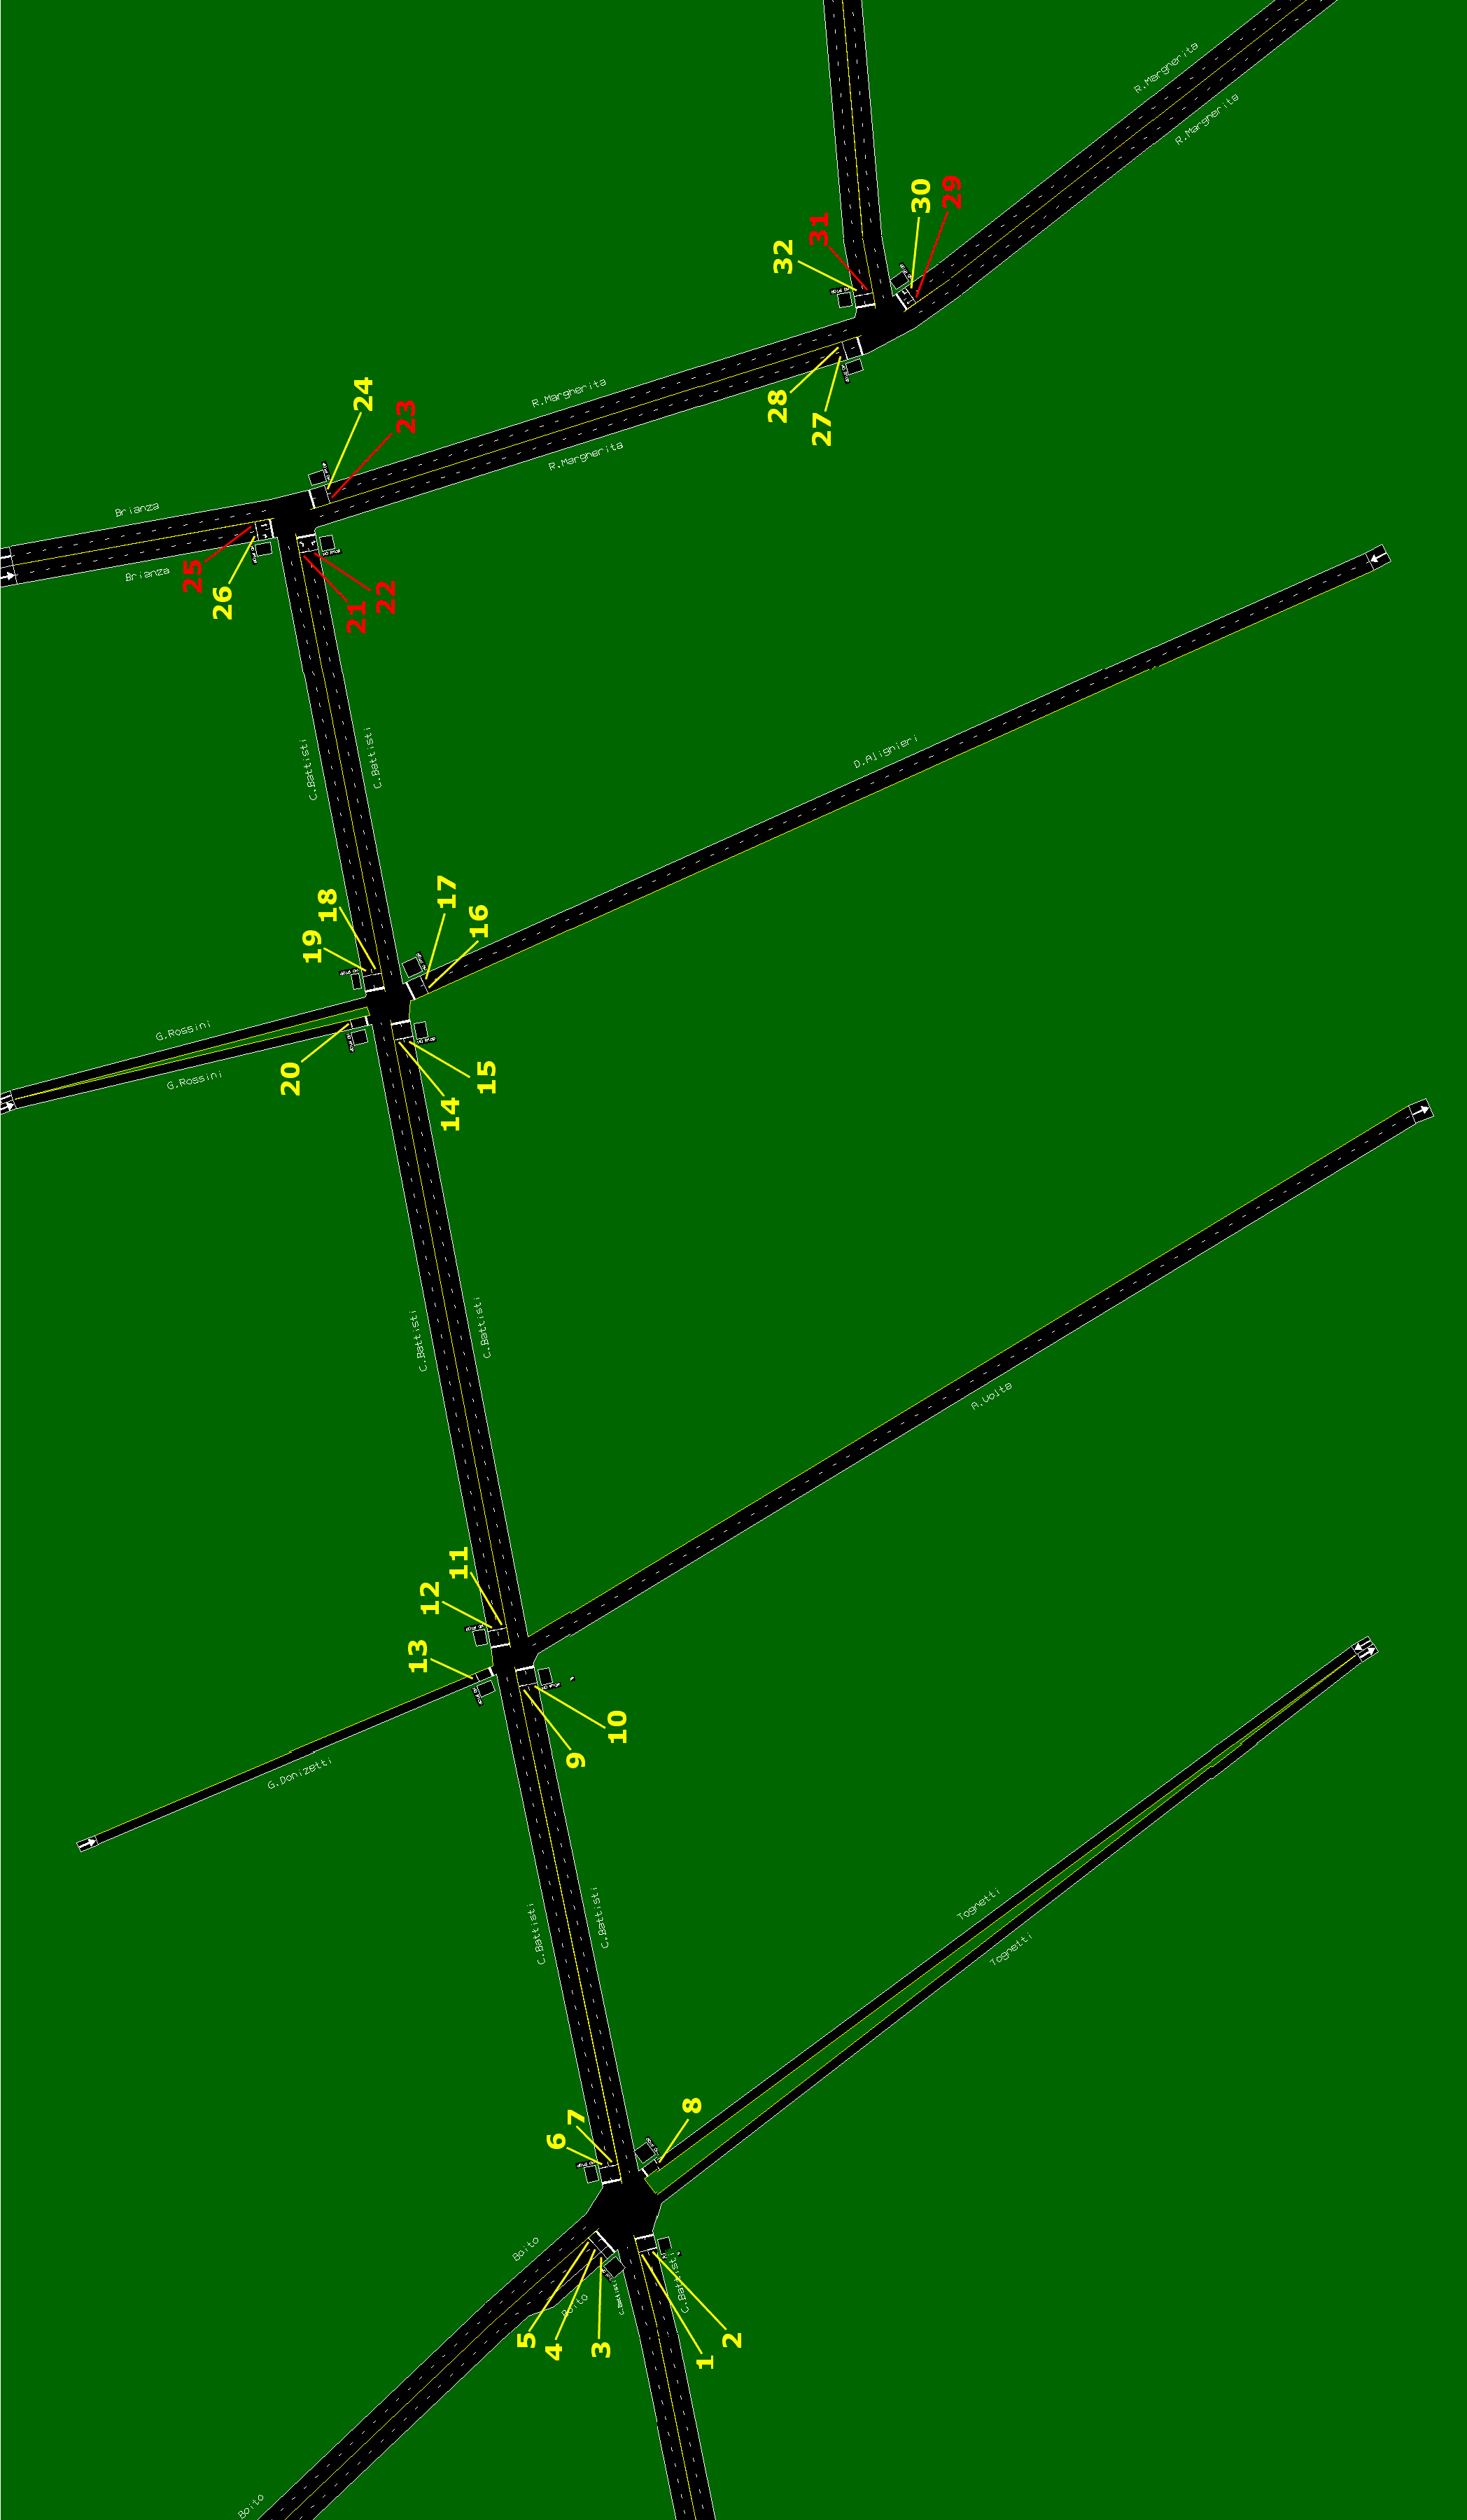
\includegraphics[width=1\columnwidth]{tsis-model-monza-compact}%
  	\caption[Rete stradale relativa al \ds{2}]{Visualizzazione del file \acs{TNO} rappresentante la rete stradale da cui viene generato il \ds{2}.}
	\label{fig:tsis-model-monza}
\end{figure}

\begin{table}[ht]%
	\centering%
	\begin{tabular}{+l^l}
	\toprule\rowstyle{\bfseries}%
	\#  & Sensore \\\otoprule
	$01$& D$782$       \\
	$02$& D$781$       \\
	$03$& D$1687$      \\
	$04$& D$1681$      \\
	$05$& D$1682$      \\
	$06$& D$981$       \\
	$07$& D$982$       \\
	$08$& D$1480$      \\\bottomrule
	\end{tabular}
	\hspace{-0.6em}
	\begin{tabular}{+l^l}
	\toprule\rowstyle{\bfseries}%
	\#  & Sensore \\\otoprule
	$09$& D$892$       \\
	$10$& D$891$       \\
	$11$& D$192$       \\
	$12$& D$191$       \\
	$13$& D$1290$      \\
	$14$& D$912$       \\
	$15$& D$911$       \\
	$16$& D$1092$      \\\bottomrule
	\end{tabular}
	\hspace{-0.6em}
	\begin{tabular}{+l^l}
	\toprule\rowstyle{\bfseries}%
	\#  & Sensore \\\otoprule
	$17$& D$1091$      \\
	$18$& D$212$       \\
	$19$& D$211$       \\
	$20$& D$110$       \\
	\color{red}$21$& D$5098*$     \\
	\color{red}$22$& D$5099*$     \\
	\color{red}$23$& D$5097*$     \\
	$24$& D$421$       \\\bottomrule
	\end{tabular}
	\hspace{-0.6em}
	\begin{tabular}{+l^l}
	\toprule\rowstyle{\bfseries}%
	\#  & Sensore \\\otoprule
	\color{red}$25$& D$5096*$     \\
	$26$& D$321$       \\
	$27$& D$241$       \\
	$28$& D$242$       \\
	\color{red}$29$& D$5094*$     \\
	$30$& D$642$       \\
	\color{red}$31$& D$5095*$     \\
	$32$& D$541$       \\\bottomrule
	\end{tabular}
	\caption[Sensori relativi al \ds{2}]{Corrispondenza fra gli identificatori dei sensori del \ds{2} e l'indice con cui essi sono indicati nella \vref{fig:tsis-model-monza}.}
	\label{tab:ds-2-sensors-indices}
\end{table}
Nella~\vref{tab:ds-2-sensors-indices}, i sensori il cui identificatore è contrassegnato da un asterisco corrispondono ai sensori reali, evidenziati anche nella \vref{fig:tsis-model-monza} tramite un indice numerico di colore rosso; i restanti sensori corrispondono a quelli aggiunti per estendere il modello in questione.

Di seguito si riportano le ulteriori caratteristiche della rete stradale oggetto di questa sottosezione:
\begin{itemize}
	\item la larghezza delle corsie è \num{3.65} \si{\metre}
	\item le strade del modello \acs{TSIS} riproducono esattamente, sia in lunghezza che in forma, la porzione di strada reale che modellano:
	\begin{itemize}
		\item \emph{Viale Battisti} è lungo \num{1.33} \si{\kilo\metre}
		\item \emph{Via Boito} è lunga \num{308} \si{\metre}
		\item \emph{Via Tognetti} è lunga \num{351} \si{\metre}
		\item \emph{Via Donizzetti} è lunga \num{176} \si{\metre}
		\item \emph{Via Volta} è lunga \num{395} \si{\metre}
		\item \emph{Via Rossini} è lunga \num{141} \si{\metre}
		\item \emph{Via Dante} è lunga \num{422} \si{\metre}
		\item \emph{Viale Brianza} è lungo \num{106} \si{\metre}
		\item \emph{Viale Margherita} è lungo \num{505} \si{\metre}
		\item \emph{Via Boccaccio} è lunga \num{336} \si{\metre}
	\end{itemize}
	\item la dimensione dei sensori è \num{0.03} \si{\metre}, da cui consegue che la dimensione della zona sensibile (in tutte le direzioni) è \num{1.85} \si{\metre}
	\item la distanza dei sensori dall'intersezione più vicina è \num{6.5} \si{\metre}
	\item la velocità media dei veicoli: \num{67} \si{km/h} su \emph{Viale Battisti}, \num{56} \si{km/h} sulle altre strade.
\end{itemize}

Come anticipato, per questo caso di studio si sono creati $3$ modelli di simulazione differenti (corrispondenti quindi a $3$ differenti sorgenti \acs{TRF}), al fine di rappresentare i diversi flussi di traffico durante la settimana.

Il file \acs{TRF} creato per modellare il traffico sulla rete stradale nei giorni lavorativi prevede un tempo di simulazione totale pari a $24$ ore, suddiviso in $12$ \emph{time period}, ognuno dei quali composto da \emph{time interval\index{dataset!time interval}} della durata di $100$ secondi: la \vref{tab:ds-2-tp-labels} illustra la durata (in ore) di ognuno di essi e introduce la corrispondenza fra essi e la fase della giornata, rappresentata come la variabile classe nel relativo dataset.

Nei modelli di traffico relativi al sabato e alla domenica la corrispondenza tra i \emph{time period}, che rimangono identici a quelli mostrati nella tabella \vref{tab:ds-2-tp-labels}, e la variabile classe è differente. Ad esempio, il \emph{time period} $1$ del modello di traffico relativo al sabato è stato associato alla classe $11$ mentre il \emph{time period} $1$ del modello di traffico relativo alla domenica è stato associato alla classe $21$. Ne deriva che gli identificatori della variabile classe per questi due modelli di traffico sono incrementati di una e due decine rispetto agli identificatori usati per il modello di traffico relativo ai giorni lavorativi.
\begin{table}[htbp]%
	\centering%
	\begin{tabular}{+l^l^l^l}
	\toprule\rowstyle{\bfseries}%
	Fascia oraria  		   & Time Period  	& Fase          & Classe  \\\otoprule
	$00$:$00$ - $02$:$05$  & $1$            & notte         & $1$     \\
	$02$:$05$ - $04$:$10$  & $2$            & notte         & $1$     \\
	$04$:$10$ - $06$:$15$  & $3$            & alba          & $2$     \\
	$06$:$15$ - $08$:$20$  & $4$            & mattino       & $3$     \\
	$08$:$20$ - $10$:$25$  & $5$            & mattino       & $3$     \\
	$10$:$25$ - $12$:$30$  & $6$            & giorno        & $4$     \\
	$12$:$30$ - $14$:$35$  & $7$            & giorno        & $4$     \\
	$14$:$35$ - $16$:$40$  & $8$            & giorno        & $4$     \\
	$16$:$40$ - $18$:$45$  & $9$            & pomeriggio    & $5$     \\
	$18$:$45$ - $20$:$50$  & $10$           & pomeriggio    & $5$     \\
	$20$:$50$ - $22$:$55$  & $11$           & sera          & $6$     \\
	$22$:$55$ - $24$:$00$  & $12$           & sera          & $6$     \\\bottomrule
	\end{tabular}
	\caption[Periodi temporali del \ds{2}]{Caratterizzazione dei periodi temporali (\ie{} \emph{time period\index{dataset!time period}}) del modello \acs{TSIS} relativo al \ds{2} (giorni lavorativi).}
	\label{tab:ds-2-tp-labels}
\end{table}

Ogni fase della giornata (\ie{} classe) è caratterizzata da un andamento diverso del traffico. Di seguito si presenta l'andamento generale del traffico durante i giorni lavorativi:
\begin{itemize}
	\item al mattino (\ie{} periodi temporali $4$ e $5$) traffico diretto verso il centro di \emph{Monza}, prevalentemente da \emph{Viale Battisti} (\ie{} nodo di ingresso $17$) e, in misura minore, da \emph{Viale Monza} (\ie{} nodo di ingresso $03$)
	\item durante il giorno (\ie{} periodi temporali $6$, $7$ e $8$) incremento del traffico verso il centro di \emph{Monza}, soprattutto da \emph{Viale Battisti}, e incremento del traffico fra \emph{Viale Boccaccio} e \emph{Viale Margherita} (\ie{} nodi $18$ e $19$)
	\item durante il pomeriggio (\ie{} periodi temporali $9$ e $10$) il flusso dei veicoli inizia a invertire la sua direzione verso \emph{Viale Battisti}; aumento del numero di veicoli diretti verso le strade laterali (\eg{} \emph{Via Donizzetti}, \emph{Via Alighieri}, \emph{Via Rossini})
	\item alla sera (\ie{} periodi temporali $11$ e $12$) traffico proveniente dal centro di \emph{Monza} diretto verso \emph{Viale Battisti} e, al contempo, diminuzione dei veicoli provenienti da \emph{Viale Brianza}
	\item durante la notte (\ie{} periodi temporali $1$ e $2$) riduzione del traffico su tutta la rete
	\item all'alba (\ie{} periodo temporale $3$) pochi veicoli circolanti sulla rete stradale, prevalentemente su \emph{Viale Battisti} dove si verifica un leggero incremento dei veicoli in ingresso.
\end{itemize}

Come detto, l'andamento del traffico è modellato variando i flussi di ingresso. La \vref{tab:ds-2-input-vehicles} illustra il numero di veicoli orari (\ie{} \si{vph}) in ingresso sulla rete stradale in relazione a ogni periodo temporale del modello di simulazione. Anche per i modelli di simulazione \acs{CORSIM} relativi a questa rete stradale si è scelto di utilizzare una distribuzione di probabilità di Erlang per governare l'immissione dei veicoli sulla rete stradale.
\begin{table}[h]
	\centering
	\begin{tabular}{+l^c^c^c^c^c^c^c^c}
	\toprule\rowstyle{\bfseries}%
	Time Period	& $19$		& $18$		& $17$		& $15$		& $14$		& $12$		& $11, 10$  & $03$		\\
				& \si{vph}	& \si{vph}	& \si{vph}	& \si{vph}	& \si{vph}	& \si{vph}  & \si{vph}	& \si{vph}	\\\otoprule
	$1$			& $150$ 	& $275$		& $375$		& $5$ 		& $5$ 		& $5$ 		& $5$ 		& $205$ 	\\
	$2$			& $25$ 		& $80$		& $105$		& $5$ 		& $5$ 		& $5$ 		& $5$ 		& $70$ 		\\
	$3$			& $96$ 		& $70$		& $325$		& $5$ 		& $5$ 		& $5$ 		& $5$ 		& $113$ 	\\
	$4$			& $350$ 	& $450$		& $1950$	& $20$ 		& $50$ 		& $20$ 		& $20$ 		& $1080$ 	\\
	$5$			& $500$ 	& $600$		& $1855$	& $20$ 		& $20$ 		& $20$ 		& $20$ 		& $1325$ 	\\
	$6$			& $750$ 	& $500$		& $2100$	& $20$ 		& $20$ 		& $20$ 		& $20$ 		& $1022$ 	\\
	$7$			& $600$ 	& $400$		& $1950$	& $20$ 		& $20$ 		& $20$ 		& $20$ 		& $1000$ 	\\
	$8$			& $700$  	& $600$		& $2390$	& $20$ 		& $20$ 		& $20$ 		& $20$ 		& $1050$ 	\\
	$9$			& $700$ 	& $510$		& $2410$	& $20$ 		& $20$ 		& $20$ 		& $20$ 		& $1010$ 	\\
	$10$		& $700$ 	& $250$		& $2275$	& $20$ 		& $12$ 		& $20$ 		& $20$ 		& $980$ 	\\
	$11$		& $370$ 	& $190$		& $1565$	& $10$ 		& $10$ 		& $10$ 		& $10$ 		& $575$ 	\\
	$12$		& $400$ 	& $75$		& $975$		& $8$ 		& $8$ 		& $10$ 		& $7$ 		& $400$ 	\\\bottomrule
	\end{tabular}
	\caption[Flussi di ingresso relativi al \ds{2}]{Numero di veicoli orari immessi nella rete stradale da ogni nodo di ingresso (colonne) del \ds{2} (giorni lavorativi) al variare del periodo temporale sulle righe.}
	\label{tab:ds-2-input-vehicles}
\end{table}

Si osservi, inoltre, che al fine di definire il succitato andamento del traffico è stata attuata un'adeguata modellazione delle percentuali di svolta in ogni intersezione. Tuttavia, a causa della complessità del modello, non è possibile riportare le variazioni delle percentuali di svolta di ogni intersezione per ogni periodo temporale.

Per chiarezza si sottolinea infine che i profili di traffico del sabato e della domenica sono stati descritti con flussi di ingresso e percentuali di svolta di diversa entità rispetto a quelli appena descritti.

\subsection{Configurazioni del dataset}\label{subsec:config-ds-2}
Eseguendo con \acsfont{Sensors} \acs{DLL} uno qualsiasi dei modelli di simulazione (\ie{} giorni lavorativi, sabato o domenica) relativi alla rete stradale presentata, si ottiene il relativo file di output che, processato tramite gli strumenti di supporto precedentemente introdotti (si veda la \vref{sec:dataset-tools}), compone un dataset utile alla classificazione dei profili di traffico\index{classificazione!profili di traffico}.

Affinché i \keyword{dataset} in questione siano perfettamente riproducibili si sono utilizzati dei file \acs{RNS}\footnote{\acs{CORSIM} supporta l'utilizzo di file \acf{RNS} per la configurazione di alcuni aspetti della simulazione: numero di esecuzioni da effettuare e semi numerici da utilizzare per la generazione stocastica di eventi.}, semplici file di testo, opportunamente formattati, da cui \acs{CORSIM} legge il numero di esecuzioni da effettuare e i semi numerici\footnote{Il \emph{seed} è un numero utilizzato per inizializzare un generatore di numeri pseudo-casuali. Condividendo tale numero e utilizzando lo stesso generatore di numeri pseudo-casuali utilizzato da \acs{CORSIM} è possibile riprodurre la stessa identica simulazione su altri calcolatori.} relativi ad alcuni aspetti stocastici della simulazione (\eg{} incidenti, tipologia di guida dei conducenti).

Di seguito si riporta il file \acs{RNS} relativo al modello di traffico per i giorni lavorativi della rete stradale illustrata nella precedente sezione.
\inputsourcecode[language=pseudo, numbers=none, caption={[Configurazione \acs{RNS} del \ds{2}]File \acs{RNS} che configura il numero di esecuzioni (\ie{} 5) e i semi numerici del modello di simulazione \acs{CORSIM} relativo alla rete stradale del \ds{2}.}, label=lst:model2-week-rns]{codes/monza-week-exte.rns}

Tralasciando i profili di traffico relativi al sabato e alla domenica, si illustrano ora le varianti generate con \acsfont{Sensors} \acs{DLL} dalla simulazione \acs{CORSIM} del profilo di traffico relativo ai giorni lavorativi. Dal modello \acs{TSIS} illustrato si sono generate $4$ diverse varianti del \ds{2} combinando la presenza o l'assenza dei sensori aggiuntivi con diversi tagli temporali dell'intero insieme di onde quadre dei sensori.

Tutte le varianti del \ds{2} generate sono accomunate dalle seguenti caratteristiche:
\begin{itemize}
	\item tempo totale pari a $86400$ secondi (\ie{} $24$ ore)
	\item la colonna \lstinline[]|tp| è stata rimossa e sostituita con la colonna \lstinline[]|class| in base alla corrispondenza riportata nella \vref{tab:ds-2-tp-labels} (gli identificatori delle classi variano, come detto, per i profili di traffico relativi al sabato e alla domenica)
	\item ogni elemento è stato ottimizzato, cioè sottoposto all'eliminazione delle righe in cui non si verifica alcuna transizione di stato dei sensori
\end{itemize}
Si osservi come tali caratteristiche siano comunque indipendenti dal profilo di traffico simulato. Le differenze tra i $3$ diversi modelli di traffico sviluppati si sostanziano nel diverso andamento dei flussi di traffico sulla rete stradale, il ché porta a diversi dati di rilevazione da parte dei sensori; nel numero di esecuzioni della simulazione (\ie{} $5$ per i giorni lavorativi e $1$ per il sabato e la domenica) e nei valori assunti dalla colonna relativa alla classe di traffico (\eg{}, classe $21$ piuttosto che classe $1$).

Si descrivono infine le varianti del \ds{2} sottoposte a sperimentazione.
\begin{description}
	\item[\ds{2\text{.}B\text{.}100}] \hfill \\
	Dataset composto da $864$ elementi (\ie{} file) ognuno dei quali rappresenta al più $100$ secondi di traiettoria\index{traiettoria} dei sensori. Contiene solamente le onde quadre relative ai $6$ sensori reali (\ie{} D$5094$, D$5095$, D$5096$, D$5097$, D$5098$ e D$5099$).
	\item[\ds{2\text{.}B\text{.}300}] \hfill \\
	Come il precedente, tale dataset contiene solo le onde quadre relative ai sensori reali. \`E composto da $288$ elementi ognuno dei quali rappresenta al più $5$ minuti di traiettorie dei succitati sensori.
	\item[\ds{2\text{.}E\text{.}100}] \hfill \\
	Dataset composto da $864$ elementi ognuno dei quali rappresenta al più $100$ secondi di traiettorie dei sensori. Poiché esso considera tutti i sensori del modello \acs{TSIS} illustrato in questa sezione, l'intestazione di ognuno dei suoi elementi è la seguente:\par
	\lstinline[]|time, class, D5096, D341, D5098, D5099, D211, D212, |\\\lstinline[]|D241, D242, D5097, D421, D5095, D541, D5094, D641, |\\\lstinline[]|D891, D892, D981, D982, D911, D912, D191, D192, D1290, |\\\lstinline[]|D1682, D1681, D1687, D1110, D1091, D1092, D1480, D781, |\\\lstinline[]|D782|.
	\item[\ds{2\text{.}E\text{.}300}] \hfill \\
	Dataset composto da $288$ elementi ciascuno dei quali rappresenta al più $5$ minuti di traiettorie dei sensori. Come il procedente, anche questo dataset, è stato generato dal modello \acs{TSIS} provvisto dei sensori aggiuntivi.
\end{description}

\cleardoublepage
\section{Sperimentazione}
In questa sezione si presentano i risultati ottenuti dalla \keyword{sperimentazione} della classe dei classificatori \acs{CTBN} (\acs{CTBNC})\index{classificazione!\acsfont{CTBNC}} descritta in questo lavoro di tesi.

Prima di presentare tali risultati si introduce la metodologia di \keyword{sperimentazione} utilizzata sui succitati $6$ dataset.

Come anticipato, dato un modello di classificatore \acs{CTBN}, si è svolta la stessa $k$-\emph{fold\index{fold|see{cross-validazione}} \keyword{cross-validazione}} con $k = 10$ per ognuno dei \keyword{dataset} generati\index{classificazione!profili di traffico}. Si è cioè suddiviso ognuno dei succitati dataset in $10$ campioni di uguale numerosità utilizzandone uno come \emph{validation set\index{validation set|see{test set}}} (\ie{} \emph{\keyword{test set}}) e i restanti come \emph{\keyword{training set}}. Quindi tale processo è stato ripetuto $10$ volte, affinché ognuno dei $10$ campioni venisse utilizzato come \emph{\keyword{test set}} esattamente una sola volta.

Il fine della \emph{\keyword{cross-validazione}} è quello di valutare la capacità di apprendimento e generalizzazione di un modello predittivo \citep[si veda][capitolo $7$]{Hastie2001}, qual è il classificatore \acs{CTBN}. La \emph{\keyword{cross-validazione}} è considerata una delle tecniche possibili utilizzabili al fine di rilevare e evitare il problema dell'\emph{\keyword{overfitting}}\footnote{Il problema dell'\emph{overfitting} è un problema frequente nei campi di ricerca che utilizzato modelli e tecniche statistiche (\eg{} apprendimento automatico, data mining). Tale problema si verifica quando un modello statistico si adatta eccessivamente al \emph{training set} perdendo così la capacità di riconoscere (\ie{} classificare, nel caso di modelli predittivi) istanze del problema non conosciute; non acquisendo cioè una adeguata capacità di generalizzazione.}. A tale scopo, i risultati di ognuno dei $10$ processi di classificazione possono essere mediati (o combinati in modi alternativi) al fine di produrre singoli valori che stimino l'efficacia\footnote{L'efficacia di un classificatore è un termine generico che indica un insieme di misure (\eg{} \emph{precision\index{precision|see{metrica}}}, \emph{recall\index{recall|see{metrica}}}, \emph{$F$-measure\index{$F$-measure|see{metrica}}} e \emph{accuracy\index{accuracy|see{metrica}}}) della qualità di un classificatore.} del modello predittivo utilizzato. In questa sperimentazione, avendo affrontato un problema di \emph{classificazione multi-classe\index{classificazione!multi-classe}}, si sono mediati i risultati relativi a ogni \emph{fold\index{cross-validazione!fold}}\footnote{Un fold\index{fold|see{cross-validazione}} indica una configurazione, comprensiva di \emph{\keyword{training set}} e \emph{\keyword{test set}}, delle $k$ utilizzate durante una $k$-\emph{fold \keyword{cross-validazione}}.} utilizzando i cosiddetti approcci \emph{\keyword{micro-average}} e \emph{\keyword{macro-average}}.

La differenza tra queste due tecniche di sintesi dei risultati consiste nel fatto che mentre l'approccio \emph{\keyword{macro-average}} è una media (non pesata) delle metriche relative ad ogni classe, l'approccio \emph{\keyword{micro-average}}, al contrario, consiste in una media delle metriche attuata sul totale delle istanze sottoposte a classificazione. Da ciò consegue che la tecnica \emph{\keyword{micro-average}} tende a conferire maggiore peso alle classi composte da più istanze e costituisce, in caso di classi popolose nel \emph{\keyword{test set}} una reale misura dell'efficacia del classificatore. Invece, per sintetizzare l'efficacia del classificatore su classi composte da poche istanze è preferibile considerare le indicazioni di efficacia date dall'approccio \emph{\keyword{macro-average}} \citep[si veda][sezione 13.6]{Manning2008}.

Si precisa che i risultati presentati di seguito sono quelli ottenuti dall'approccio \emph{\keyword{micro-average}} poiché le classi dei dataset generati sono tutte composte da numeri di istanze comparabili e nessuna di esse domina le altre in termini quantitativi.

Inoltre, si specifica che le procedure di apprendimento dei parametri di ogni classificatore \acs{CTBN} (\acs{CTBNC}) appreso sono state effettuate utilizzando la \emph{stima bayesiana} (si veda l'intera \autoref{subsec:ctbn-params} \vpageref{subsec:ctbn-params}) con \keyword{conteggi immaginari} $\alpha_{\setel{x}\setel{x}^{\prime}}$ e $\tau_{\setel{x}}$ impostati rispettivamente ai valori $1$ e $0.005$.

La procedura di \keyword{sperimentazione} descritta è stata attuata per i $4$ differenti modelli di classificatori \acs{CTBN} elencati di seguito:
\begin{itemize}
	\item classificatore \acs{CTNB} (\acs{CTNBC})
	\item classificatore \acs{CTBN} appreso dal \emph{\keyword{training set}} (tramite la procedura di apprendimento strutturale presentata nel \vref{cap:structurallearning}) fissando il numero massimo di genitori a $2$
	\item classificatore \acs{CTBN} appreso dal \emph{\keyword{training set}} fissando il numero massimo di genitori a $3$
	\item classificatore \acs{CTBN} appreso dal \emph{\keyword{training set}} fissando il numero massimo di genitori a $4$.
\end{itemize}
L'obiettivo delle prossime sezioni è quindi quello di comparare l'efficacia di tali classificatori.

\subsection{Metriche di valutazione}
Prima di presentare i risultati relativi ai succitati classificatori si illustra la metodologia con cui si sono state calcolate le metriche di valutazione per ognuna delle $6$ sperimentazioni effettuate.

Come anticipato, dato uno qualunque dei dataset generati si è configurata per esso una sperimentazione $k$-\emph{fold \keyword{cross-validazione}} con $k$ = 10.

Ottenuti i risultati relativi ai processi di classificazione, per ognuno dei $10$ \emph{fold\index{cross-validazione!fold}} si è effettuato il processo di \emph{\keyword{cross-tabulazione}}\footnote{Il processo di \keyword{cross-tabulazione} consiste in un processo statistico il cui scopo è riassumere le interrelazioni che intercorrono fra due variabili categoriche dei dati. L'output di questo processo corrisponde solitamente a una \emph{matrice di confusione\index{matrice!confusione, di}}.} tra le classi reali delle istanze e le classi ad esse assegnate dal processo di \emph{classificazione supervisionata\index{classificazione!supervisionata}}. Calcolate così le \emph{matrici di confusione\index{matrice!confusione, di}}, si è proceduto alla computazione delle metriche di valutazione per ogni \emph{fold\index{cross-validazione!fold}} e successivamente all'effettuazione delle medie \emph{\keyword{macro-average}} e \emph{\keyword{micro-average}}.

La \vref{tab:contingency-table} riproduce un esempio di \emph{matrice di confusione\index{matrice!confusione, di}} calcolata per ogni singolo processo di classificazione. Essa rappresenta le classi reali delle istanze sulle colonne e le classi inferite sulle righe. Ogni cella $(i\,,\,j)$ contiene il numero di istanze della classe $j$ classificate come appartenenti alla classe $i$. Ne deriva perciò che una classificazione perfetta (il ché, si noti, non corrisponde a aver appreso un classificatore perfetto) corrisponde ad una matrice diagonale\footnote{Una matrice diagonale è una matrice quadrata in cui solamente i valori della diagonale principale sono diversi da $0$.}.
\begin{table}[ht]
	\footnotesize
	\centering%
	\begin{tabular}{+c^c^c^c^c^c^c}
	\toprule\rowstyle{\bfseries}%
		    		& Classe $1$ & Classe $2$ & Classe $3$ & Classe $4$ & Classe $5$ & Classe $6$ \\\otoprule
    \bfseries{Classe $1$} 	& $(1\,,\,1)$ & $(1\,,\,2)$ & $(1\,,\,3)$ & $(1\,,\,4)$ & $(1\,,\,5)$ & $(1\,,\,6)$ \\
    \bfseries{Classe $2$} 	& $(2\,,\,1)$ & $(2\,,\,2)$ & $(2\,,\,3)$ & $(2\,,\,4)$ & $(2\,,\,5)$ & $(2\,,\,6)$ \\
    \bfseries{Classe $3$} 	& $(3\,,\,1)$ & $(3\,,\,2)$ & $(3\,,\,3)$ & $(3\,,\,4)$ & $(3\,,\,5)$ & $(3\,,\,6)$ \\
    \bfseries{Classe $4$} 	& $(4\,,\,1)$ & $(4\,,\,2)$ & $(4\,,\,3)$ & $(4\,,\,4)$ & $(4\,,\,5)$ & $(4\,,\,6)$ \\
    \bfseries{Classe $5$} 	& $(5\,,\,1)$ & $(5\,,\,2)$ & $(5\,,\,3)$ & $(5\,,\,4)$ & $(5\,,\,5)$ & $(5\,,\,6)$ \\
    \bfseries{Classe $6$} 	& $(6\,,\,1)$ & $(6\,,\,2)$ & $(6\,,\,3)$ & $(6\,,\,4)$ & $(6\,,\,5)$ & $(6\,,\,6)$ \\\bottomrule
    \end{tabular}
    \caption[Matrice di confusione\index{matrice di confusione} multi-classe]{Esempio di \emph{matrice di confusione\index{matrice!confusione, di}} specifico del problema di \emph{classificazione multi-classe\index{classificazione!multi-classe}} affrontato.}\label{tab:contingency-table}
\end{table}
\normalsize

A partire dalla \vref{tab:contingency-table}, per ognuna delle classi, è possibile calcolare una ulteriore \emph{matrice di confusione\index{matrice!confusione, di}} che riassumi la classificazione delle istanze appartenenti ad una singola classe piuttosto che alle altre (approccio detto \virgolette{\emph{one versus all}}). La \vref{tab:contingency-table-single-class} di seguito riporta un esempio di tale matrice. Fissata una classe, tale tabella, tramite alcune metriche di base che si descrivono di seguito, mette in relazione le classi reali delle istanze con le rispettive classi inferite.
\begin{table}[ht]
	\centering
	\begin{tabular}{+c^c^c^c}
	\toprule\rowstyle{\bfseries}%
	Inferite $\downarrow$ / Reali $\rightarrow$	& Positivi & Negativi & 			\\\otoprule
	\bfseries{Positivi} 						& \acs{TP} & \acs{FP} & \acs{PPV}	\\
	\bfseries{Negativi} 						& \acs{FN} & \acs{TN} & \acs{NPV} 	\\
												& \acs{TPR}& \acs{TNR}& 			\\\bottomrule
	\end{tabular}
	\caption[Esempio di matrice di confusione]{Esempio di matrice di confusione\index{matrice!confusione, di} relativa al processo di classificazione di una singola classe.}\label{tab:contingency-table-single-class}
\end{table}

Si osservi che la computazione di tali matrici di confusione è un passo necessario al calcolo delle medie \emph{\keyword{macro-average}}, ottenute appunto dalle metriche relative alle singole classi. Invece, come detto, per il calcolo delle medie \emph{\keyword{micro-average}} si procede sul totale delle istanze del \emph{\keyword{test set}}.

Di seguito si elencano e presentano le metriche di valutazione calcolate.
\begin{description}
	\item[True Positive] \hfill \\
	Il valore della metrica \acf{TP}\index{metrica!true positive} corrisponde al numero di istanze classificate correttamente.
	\item[True Negative] \hfill \\
	Il valore della metrica \acf{TN}\index{metrica!true negative} corrisponde al numero di istanze non appartenenti alla classe corrente classificate correttamente (\eg{} numero di istanze non appartenenti alla classe $1$ che sono state classificate come appartenenti a un'altra classe).
	\item[False Positive] \hfill \\
	Il valore della metrica \acf{FP}\index{metrica!false positive} corrisponde al numero di istanze non classificate correttamente.
	\item[False Negative] \hfill \\
	Il valore della metrica \acf{FN}\index{metrica!false negative} corrisponde al numero di istanze non appartenenti alla classe corrente ma classificate come tali (\eg{} numero di istanze non appartenenti alla classe $1$ ma classificate come tali).
	\item[True Positive Rate] \hfill \\
	Il \acf{TPR}\index{metrica!true positive rate}, detto anche \emph{recall}\index{metrica!recall} o \emph{sensitivity}\index{metrica!sensitivity}, esprime l'abilità del modello nel classificare le istanze in modo corretto. \`E così calcolato:\par
	\[TPR=\frac{TP}{TP + FN} = 1 - FNR\text{.}\]
	\item[False Negative Rate] \hfill \\
	Il \acf{FNR}\index{metrica!false negative rate} è l'inverso della metrica \acs{TPR}. \`E quindi calcolato nel seguente modo:\par
	\[FNR=\frac{FN}{TP + FN} = 1 - TPR\text{.}\]
	\item[True Negative Rate] \hfill \\
	Il \acf{TNR}\index{metrica!true negative rate}, detto anche \emph{specificity\index{metrica!specificity}}, misura l'abilità del modello nel non sbagliare classificazione, cioè nell'identificare le istanze da non classificare come appartenenti alla classe in esame. \`E così calcolato:\par
	\[TNR=\frac{TN}{TN + FP} = 1 - FPR\text{.}\]
	\item[False Positive Rate] \hfill \\
	Il \acf{FPR}\index{metrica!false positive rate}, detto anche \emph{false alarm rate\index{metrica!false alarm rate}} o \emph{fall-out\index{metrica!fall-out}}, è l'inverso della metrica \acs{TNR}. \`E calcolato nel seguente modo:\par
	\[FPR = \frac{FP}{TN + FP} = 1 - TNR\text{.}\]
	\item[Positive Predictive Value] \hfill \\
	Il \acf{PPV}\index{metrica!positive predictive value}, detto anche \emph{precision\index{metrica!precision}}, rappresenta la proporzione delle istanze classificate correttamente. Esso è calcolato come segue:
	\[PPV = \frac{TP}{TP + FP} = 1 - FDR\text{.}\]
	\item[Negative Predictive Value] \hfill \\
	Il \acf{NPV}\index{metrica!negative predictive value} è una metrica che rappresenta la proporzione delle istanze correttamente classificate come non appartenenti a quella in esame. \`E calcolato nel seguente modo:\par
	\[NPV = \frac{TN}{TN + FN}\text{.}\]
	\item[F-Measure] \hfill \\
	Il punteggio \acf{F1}\index{metrica!$F$-measure} è una misura dell'accuratezza che un modello possiede. Nello specifico esso consiste nella media armoncia delle metriche \emph{precision\index{precision|see{metrica}}} e \emph{recall\index{recall|see{metrica}}}:
	\[F_1 = 2 \cdot \frac{PPV \cdot TPR}{PPV + TPR}\text{.}\]
	\item[Accuratezza] \hfill \\
	L'accuratezza di un modello (\ie{} \emph{accuracy\index{metrica!accuracy}}), intesa come la sua capacità di classificare correttamente tutte le istanze (che appartengano o meno alla classe in esame), è computata nel seguente modo:
	\[ACC = \frac{TP + TN}{TP + TN + FP + FN}\text{.}\]
\end{description}
Per la computazione delle metriche sono stati usati intervalli di confidenza al $90$\%.

A titolo informativo si comunica che l'implementazione di quanto descritto in questa sottosezione è stata attuata con l'ausilio di una libreria \lstinline$R$, il pacchetto \lstinline$caret$ \citep{CARET2013}.

\subsection{Accuratezza}
In questa sottosezione si presentano i risultati dei processi di \emph{classificazione supervisionata} dei $6$ dataset effettuati per ognuno dei $4$ modelli di classificatori presi in considerazione. Per ogni dataset sottoposto a sperimentazione si illustra e commenta il valore della metrica \emph{accuracy\index{metrica!accuracy}} relativo ad ognuno dei classificatori utilizzati. Si rimarca che la metrica \emph{accuracy\index{metrica!accuracy}} è stata calcolata tramite approccio \emph{\keyword{micro-average}} su tutti i \emph{fold\index{cross-validazione!fold}} di ogni sperimentazione\index{risultati!sperimentazione}.
\cleardoublepage
\begin{table}
	\centering
	\begin{tabular}{+l^c^c^c^c}
	\toprule\rowstyle{\bfseries}%
				   				& \acs{CTNBC} 			& \acs{CTBNC}$2$ & \acs{CTBNC}$3$ 	 	& \acs{CTBNC}$4$ 		\\\otoprule
    \Ds{1\text{.}100} 			& $0.9108$ 	  			& $0.9236$       & \color{red}$0.9259$ 	& \color{red}$0.9259$ 	\\
    \Ds{1\text{.}300}   		& \color{red}$0.9548$ 	& $0.9513$       & $0.9513$ 			& $0.9513$				\\
    \Ds{2\text{.}B\text{.}100} 	& \color{red}$0.6254$	& $0.6250$       & $0.6233$       		& $0.6206$          	\\
    \Ds{2\text{.}B\text{.}300} 	& \color{red}$0.7159$   & $0.7013$       & $0.7013$ 			& $0.7020$ 				\\
    \Ds{2\text{.}E\text{.}100} 	& \color{red}$0.7502$ 	& $0.7270$       & $0.7307$       		& $0.7231$				\\
    \Ds{2\text{.}E\text{.}300} 	& \color{red}$0.8208$   & $0.7861$       & $0.7881$       		& $0.7791$				\\\bottomrule
	\end{tabular}
	\caption[Accuratezza dei classificatori \acs{CTBN} e \acs{CTNB}]{Comparazione del valore di \emph{accuracy\index{risultati!accuracy}} ottenuto dal classificatore \acs{CTNB} e dai classificatori \acs{CTBN} (appresi con numero massimo di genitori variabile da $2$ a $4$) su ognuno dei $6$ dataset generati. In rosso i valori maggiori per ogni dataset.}\label{tab:accuracies-table}
\end{table}

\begin{figure}
	\centering
	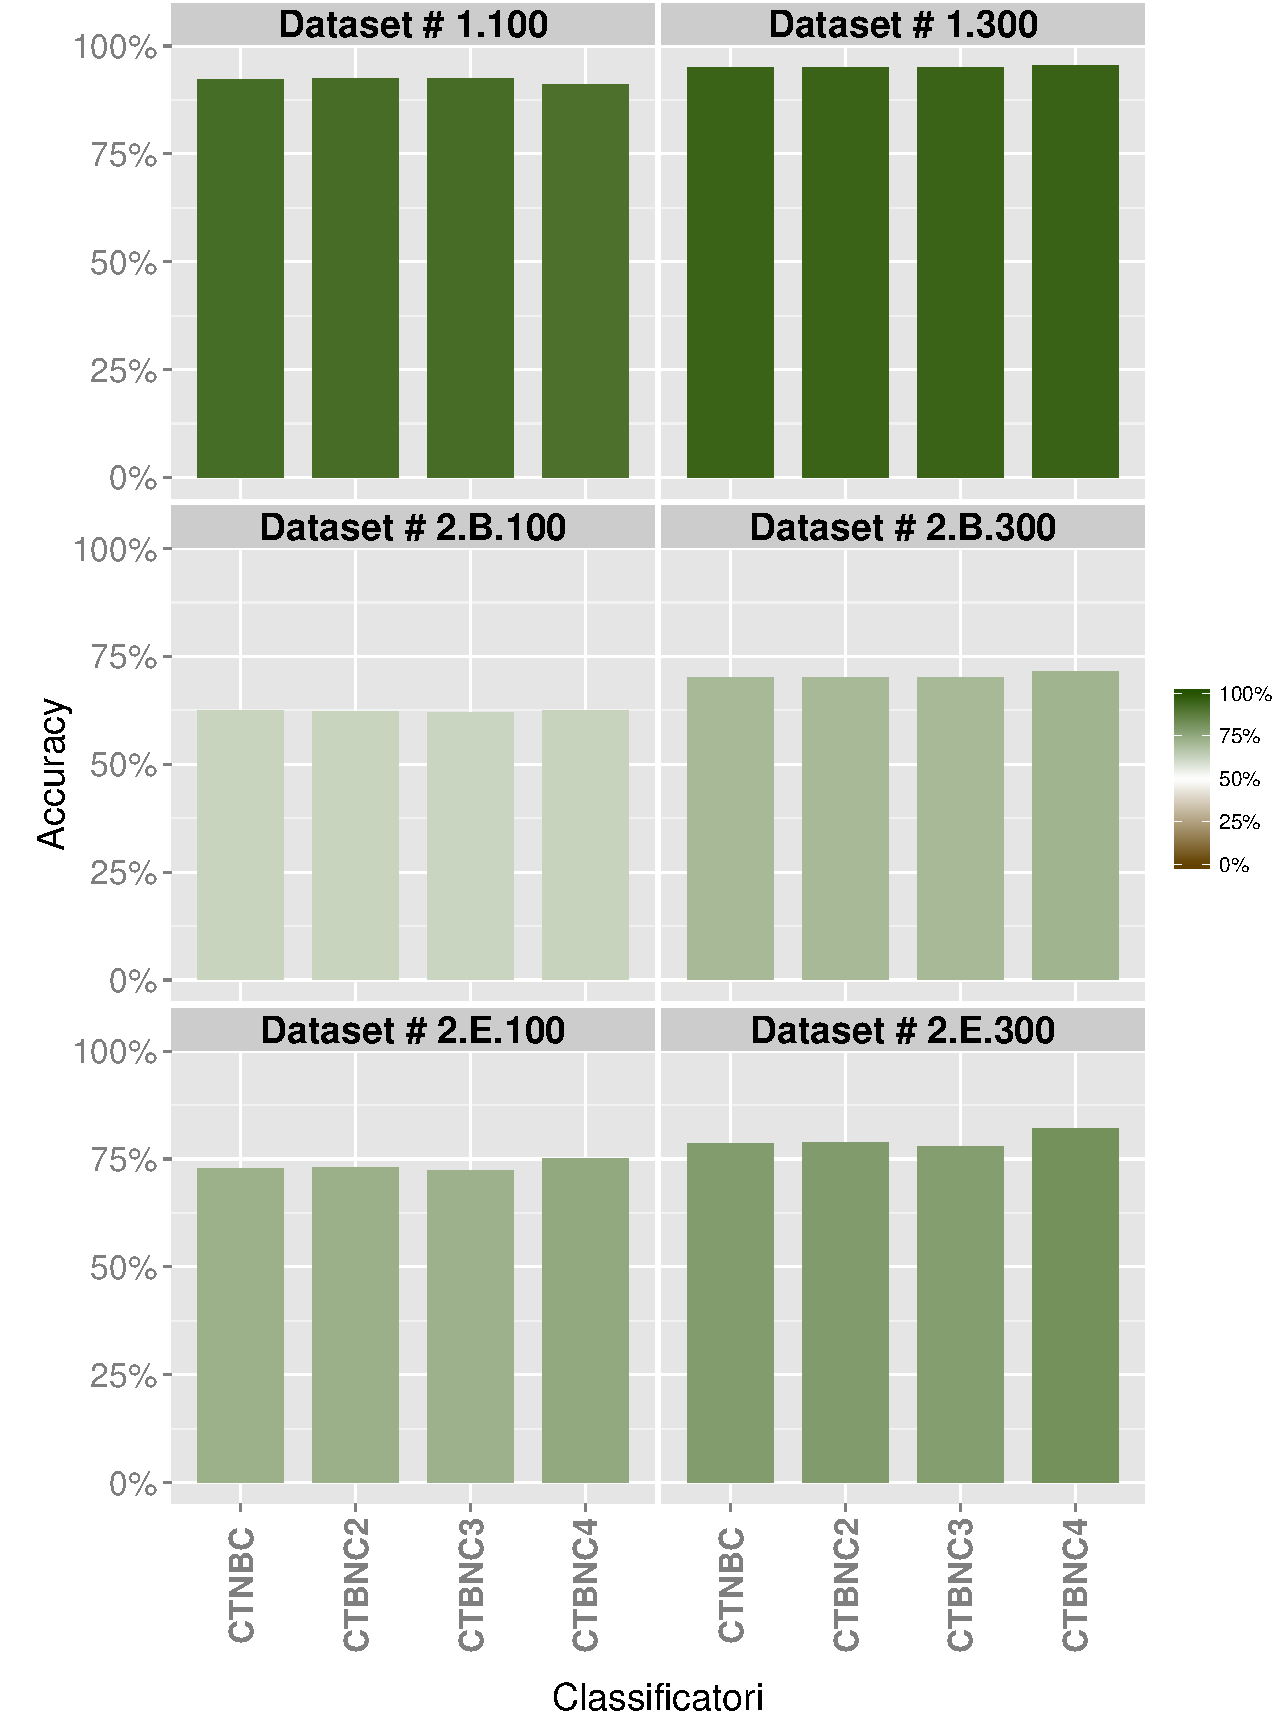
\includegraphics[width=1.3\textwidth,center]{accuracies-by-ds-by-classifier-green.pdf}
	\caption[Accuratezza dei classificatori \acs{CTBN} e \acs{CTNB}]{Comparazione del valore di \emph{accuracy\index{risultati!accuracy}} ottenuto dal classificatore \acs{CTNB} e dai classificatori \acs{CTBN} (appresi con numero massimo di genitori variabile da $2$ a $4$) su ognuno dei $6$ dataset generati.}\label{fig:accuracies-fig}
\end{figure}
%\begin{figure}
%	\centering
%	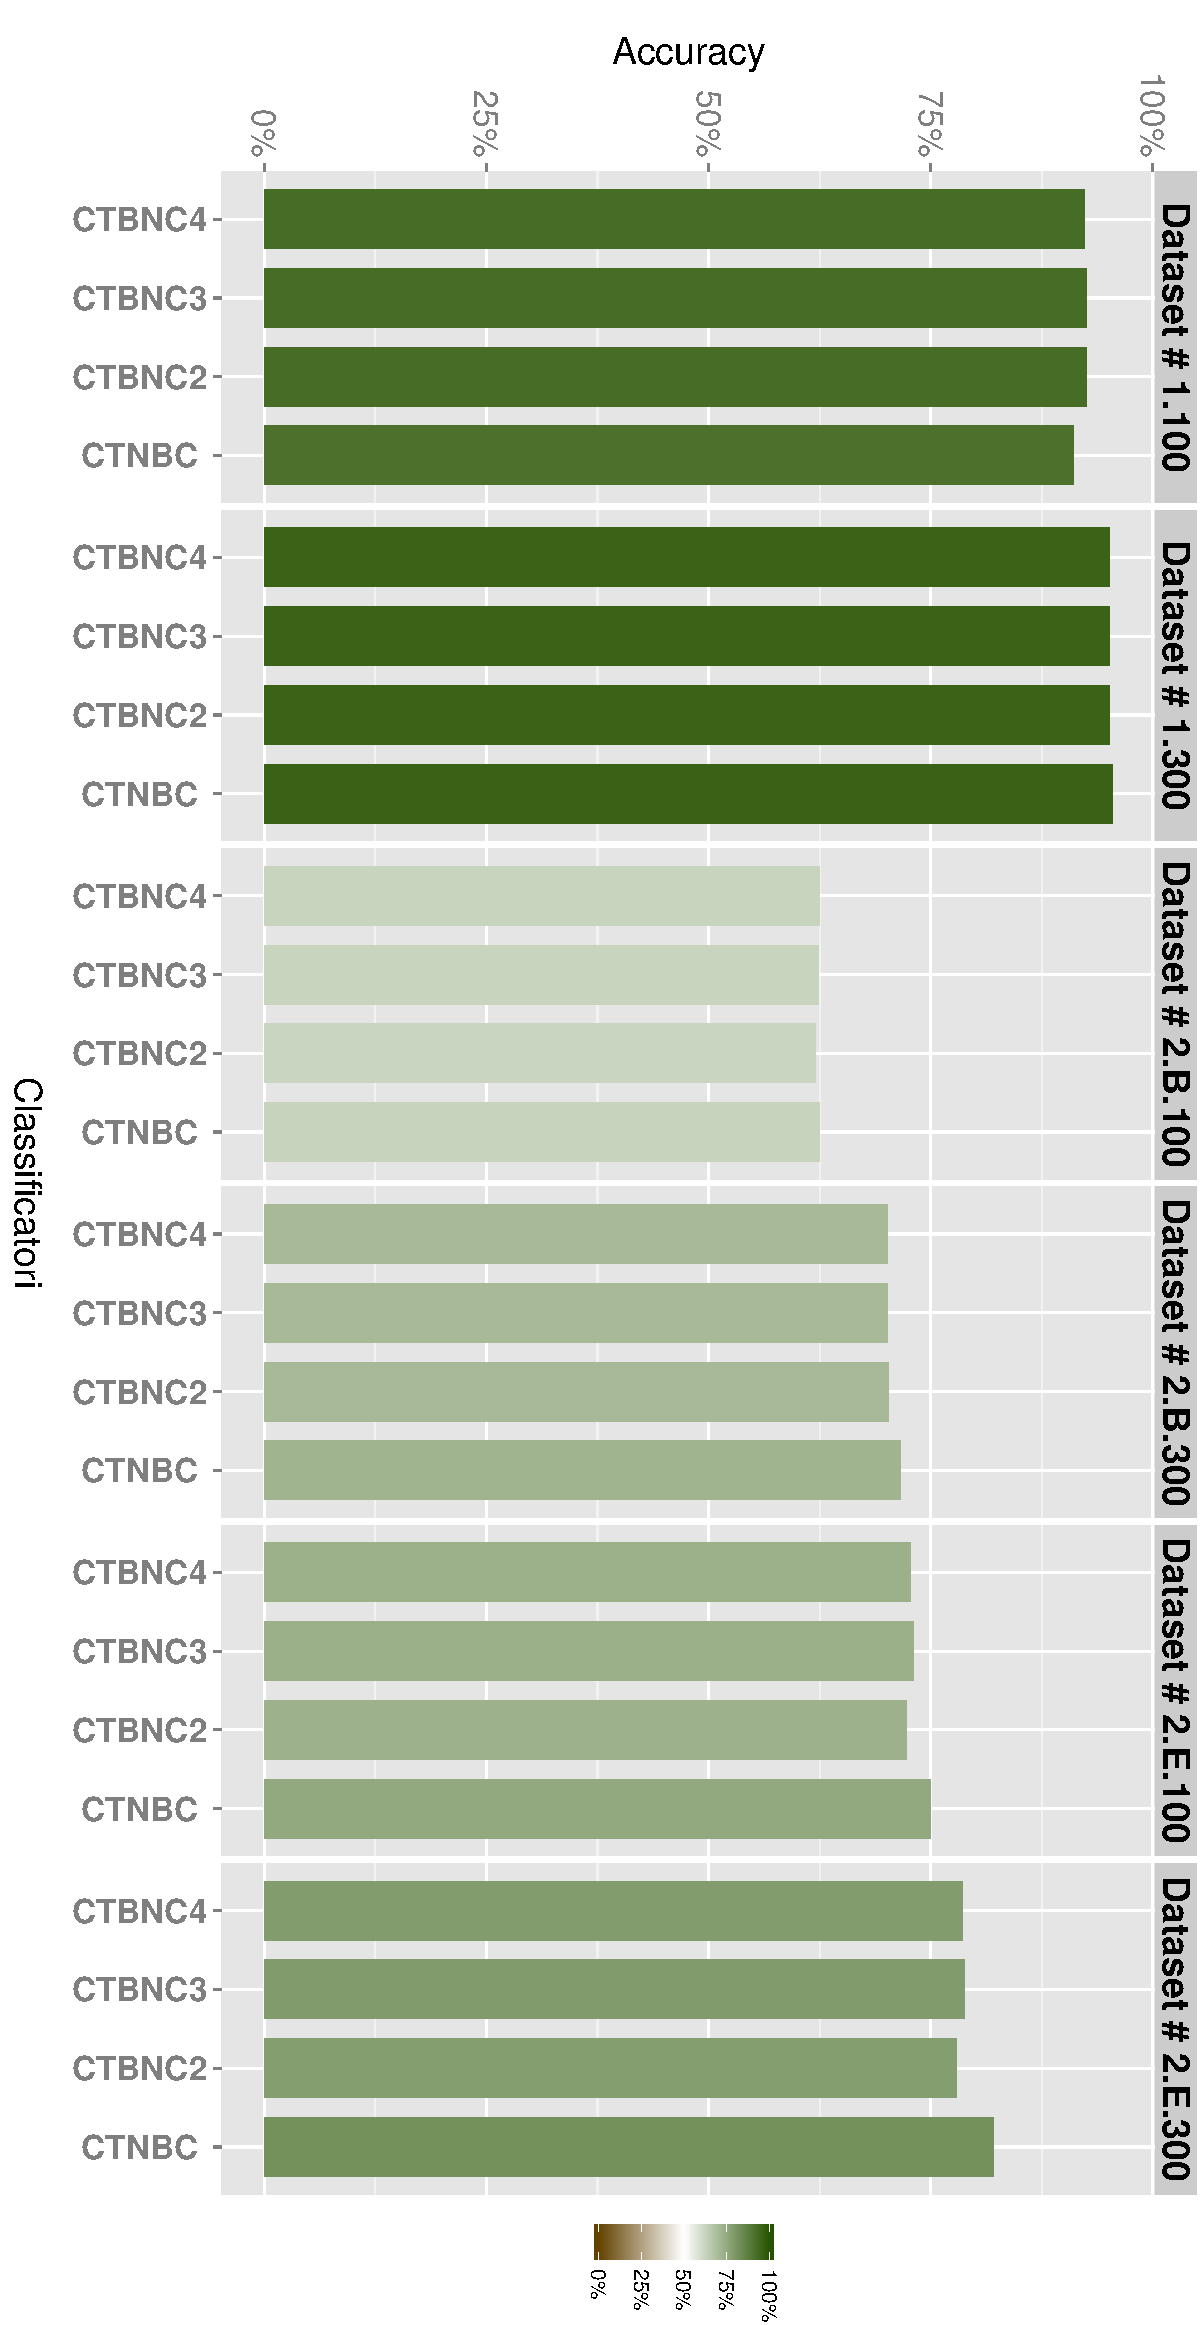
\includegraphics[width=\columnwidth,height=\textheight,keepaspectratio]{accuracies-by-ds-by-classifier-green-vert.pdf}
%	\caption[zzz]{zzz}
%\end{figure}
Seppur la \vref{tab:accuracies-table} evidenzi come il classificatore \acs{CTNB} (\acs{CTNBC}) risulti essere, per $5$ dataset su $6$, maggiormente accurato rispetto ai classificatori \acs{CTBN} appresi tramite apprendimento strutturale, è necessario osservare come tale vantaggio corrisponda in realtà a un'accuratezza superiore a quella degli altri modelli solo alla seconda o addirittura terza cifra decimale. Tale considerazione vale anche per il \ds{1\text{.}100} laddove sono i classificatori \acs{CTBN} con $k$ (\ie{} massimo numero di genitori) pari a $3$ e $4$ a riportare un leggero incremento della metrica \emph{accuracy\index{risultati!accuracy}}.

Perciò, non essendoci un classificatore che sia apprezzabilmente più accurato degli altri, possiamo asserire che i $4$ classificatori utilizzati ottengono pressappoco gli stessi risultati in termini di accuratezza della classificazione.

Tuttavia, osservando la \vref{fig:accuracies-fig} è possibile dedurre una serie di considerazioni ulteriori.

Infatti, da tale figura è possibile notare come, per ogni dataset, all'aumentare dell'intervallo temporale rappresentato dalle istanze (\ie{} $100$ secondi contro $300$), aumenti anche il livello di accuratezza della classificazione per tutti i classificatori. Tale comportamento dei classificatori è giustificabile: la suddivisione di un dataset in istanze che rappresentano un determinato intervallo temporale di dati comporta necessariamente la perdita delle transizioni di stato a cavallo fra le istanze. Ciò è correlato al comportamento descritto: i dataset le cui istanze rappresentano al più $300$ secondi di dati, essendo queste più lunghe, hanno conservato un maggior numero di transizioni di stato. Se ne deduce perciò che l'incremento di accuratezza del processo di classificazione supervisionata\index{classificazione!supervisionata} per i dataset da $300$ secondi è correlato a un aspetto quantitativo dell'informazione contenuta da tali dataset. Più semplicemente possiamo affermare che l'accuratezza dei classificatori è proporzionale all'aumento dell'intervallo temporale rappresentato dalle istanze dei dataset.

L'osservazione appena riportata è facilmente riscontrabile soprattutto osservando le due varianti del \ds{2\text{.}B} nella \autoref{fig:accuracies-fig}: il \ds{2\text{.}B\text{.}100} e il \ds{2\text{.}B\text{.}300}.

Riguardo i $2$ dataset appena citati, inoltre, è possibile notare come il livello generale di accuratezza che tutti i classificatori ottengono per essi sia ben inferiore rispetto a quello ottenuto sugli altri dataset. Anche in questo caso, si ritiene che ciò sia dovuto a un aspetto informativo dei dataset. Infatti, le istanze del \ds{2\text{.}B\text{.}100} e del \ds{2\text{.}B\text{.}300} contengono solamente le traiettorie relative ai $6$ sensori reali del \ds{2} (si veda la \autoref{subsec:config-ds-2} \vpageref{subsec:config-ds-2}).

Infine, è possibile notare come l'accuratezza dei classificatori tenda a degradare all'aumentare della complessità del sistema dinamico rappresentato dal dataset. Infatti, la differenza tra il livello di accuratezza ottenuto per il \ds{1} e quello ottenuto per il \ds{2} è significativa, tanto quanto è significativa la differenza del livello di complessità delle reti stradali che essi rappresentano.

\subsection{Curve ROC\index{\acsfont{ROC}|see{metrica}}}
L'obiettivo che questa sottosezione si prefigge è quello di completare la presentazione dei risultati ottenuti dalla sperimentazione\index{risultati!sperimentazione} dei classificatori \acs{CTBN} (\acs{CTBNC}). A tale scopo si presentano e comparano le curve \acf{ROC}\index{metrica!\acsfont{ROC}} di ogni classificatore utilizzato per la sperimentazione (\ie{} \acs{CTNBC}, \acs{CTBNC}$2$, \acs{CTBNC}$3$ e \acs{CTBNC}$4$).

Prima di tale discussione, tuttavia, è necessario introdurre i concetti relativi alla metrica \acs{ROC}\index{metrica!\acsfont{ROC}}. La visualizzazione della metrica \acs{ROC} di uno o più classificatori è una tecnica finalizzata alla valutazione e alla comparazione dell'efficacia dei classificatori. La metrica \acs{ROC} raffigura la correlazione, e spesso il \emph{tradeoff}, tra il valore della metrica \emph{recall\index{metrica!recall}} (\ie{} \emph{sensitivity\index{metrica!sensitivity}}) e il tasso di falsi positivi (\ie{} \emph{false alarm error\index{metrica!false alarm error}}; metrica \acs{FPR}).

Questa metrica, inizialmente utilizzata in altri campi di ricerca (\eg{} teoria delle decisioni), è sempre più frequentemente utilizzata anche nel campo dell'apprendimento automatico. Ciò poiché l'utilizzo della sola \emph{accuracy} come metrica per la valutazione dell'efficacia dei classificatori si rivela spesso carente dal punto di vista informativo e perciò inadeguato \citep[per approfondimenti si veda][]{Provost1997,Provost2001}.

Inoltre, la metrica \acs{ROC} gode di una serie di proprietà utili nel caso di situazioni molto comuni nel mondo reale (\eg{} insensibilità all'asimmetria delle classi): essa disaccoppia la valutazione dell'efficacia del classificatore dalla presenza o meno di classi asimmetriche o di funzioni di costo sbilanciate.

I grafici \acs{ROC} sono grafici bidimensionali la cui ordinata riporta i valori assunti dalla metrica \acs{TPR}\index{metrica!true positive rate} mentre l'ascissa riporta i valori assunti dalla metrica \acs{FPR}\index{metrica!false positive rate}.

Si osservi quindi che un grafico \acs{ROC}\index{metrica!\acsfont{ROC}} è un tipico grafico raffigurante il \emph{tradeoff} tra costi (\ie{} \acs{FPR}) e benefici (\ie{} \acs{TPR}).

Si presentano di seguito alcuni punti chiave di ogni grafico \acs{ROC}.
\begin{itemize}
	\item il punto con coordinate $(0,0)$ rappresenta il caso in cui il classificatore non commette mai errori di primo tipo (\ie{} \acf{FP}) ma nemmeno classifica positivamente le istanze (\ie{} \acf{TP})
	\item il punto con coordinate $(1,1)$ rappresenta la situazione opposta alla precedente: il classificatore classifica tutte le istanze in modo positivo, anche quelle che dovrebbe invece rigettare
	\item il punto $(0,1)$ rappresenta la classificazione perfetta.
\end{itemize}
L'interpretazione dei punti nei grafici \acs{ROC} può essere informalmente descritta in base alla loro posizione: un punto più a nord-est rispetto agli altri rappresenta una classificazione migliore. Si osservi che tale considerazione deriva dal fatto che tale punto avrebbe un'ordinata maggiore degli altri, e quindi un più alto valore \acs{TPR}, e al contempo un'ascissa inferiore, cioè un valore \acs{FPR} inferiore.

\`E bene precisare che, nel caso di \emph{classificatori probabilistici}, quali sono i classificatori \acs{CTBN}, è necessario trasformarli in \emph{classificatori discreti} (\ie{} classificatori che non forniscono un valore di probabilità come risultato bensì valori di verità) al fine di ottenere un singolo punto nello spazio del grafico \acs{ROC}\index{metrica!\acsfont{ROC}} (il quale corrisponde ad un unica \emph{matrice di confusione\index{matrice!confusione, di}}). Idealmente tale processo è svolto variando un valore di soglia in un intervallo. Per ogni soglia, si seleziona un esito positivo o negativo della classificazione in base alla probabilità restituita dal classificatore probabilistico; cioè qualora essa sia maggiore o minore del corrente valore soglia. Così facendo si ottiene quindi una curva \acs{ROC} per un qualsiasi classificatore probabilistico.

Si noti che la procedura appena descritta non è computazionalmente efficiente. Tuttavia in letteratura sono state presentate procedure efficienti \citep[si veda][sezione $5$]{Fawcett2006}.

Nel caso di un problema di \emph{classificazione multi-classe\index{classificazione!multi-classe}}, come illustrato precedentemente, la \emph{matrice di confusione\index{matrice!confusione, di}} corrisponde a una matrice $n \times n$ (in questo caso $n=6$ per tutti i dataset generati, come mostrato dalla \vref{tab:contingency-table}) contenente le $n$ classificazioni corrette (\ie{} benefici) sulla diagonale e i $n^2 - n$ possibili errori (\ie{} costi) nelle celle non sulla diagonale. Un possibile approccio risolutivo a tale problema consiste nel produrre $n$ differenti grafici \acs{ROC}, uno per classe \citep{Fawcett2006}. Per le sperimentazioni effettuate in questo lavoro di tesi si è appunto attuato tale approccio. Anche se, come già specificato, le classi dei dataset generati non presentano asimmetrie quantitative considerevoli, è tuttavia necessario notare che tale approccio provoca la perdita della proprietà di insensibilità all'asimmetria delle classi delle metriche \acs{ROC}.

Si rimarca infine che le metriche \acs{ROC} sono state calcolate tramite l'approccio \emph{\keyword{micro-average}}.

Le \vref{fig:roc-curves-class-1,fig:roc-curves-class-2,fig:roc-curves-class-3,fig:roc-curves-class-4,fig:roc-curves-class-5,fig:roc-curves-class-6} riportano i grafici delle curve \acs{ROC} di ognuno dei $4$ classificatori utilizzati per la classificazione del \ds{1\text{.}100}. Ognuna di tali figure, come detto, è relativa alla curva \acs{ROC} di una classe del dataset in questione.

Si osservi che nessuna curva \acs{ROC}\index{risultati!\acsfont{ROC}} dei classificatori differisce dalle altre in modo significativo. Al contempo, si osservi che poiché esse si avvicinano considerevolmente alla coordinata $(0,1)$ ciò indica che tutti i classificatori, in questo caso, raggiungono degli ottimi livelli di classificazione.

Il fatto che i classificatori \acs{CTBN} appresi non ottengano risultati che si discostino considerevolmente (né in positivo, né in negativo) da quelli ottenuti dal classificatore \acs{CTNB} è, con tutta probabilità, da attribuire alla complessità dei sistemi dinamici rappresentati dai dataset relativi al traffico. Con tali dataset, i classificatori appresi con la procedura di apprendimento strutturale descritta in questo lavoro di tesi, ricevono una penalità dovuta alla loro eccessiva aderenza alle interrelazioni presenti nei modelli di traffico rappresentati.

\citet{Codecasa2013} hanno infatti mostrato come l'apprendimento strutturale costituisca una procedura sensata per questa classe di modelli poiché i classificatori \acs{CTBN} appresi tramite una diverso approccio (\ie{} basato sulla log-likelihood condizionale) risultano essere maggiormente efficaci .

\begin{figure}[ht]
	\centering
	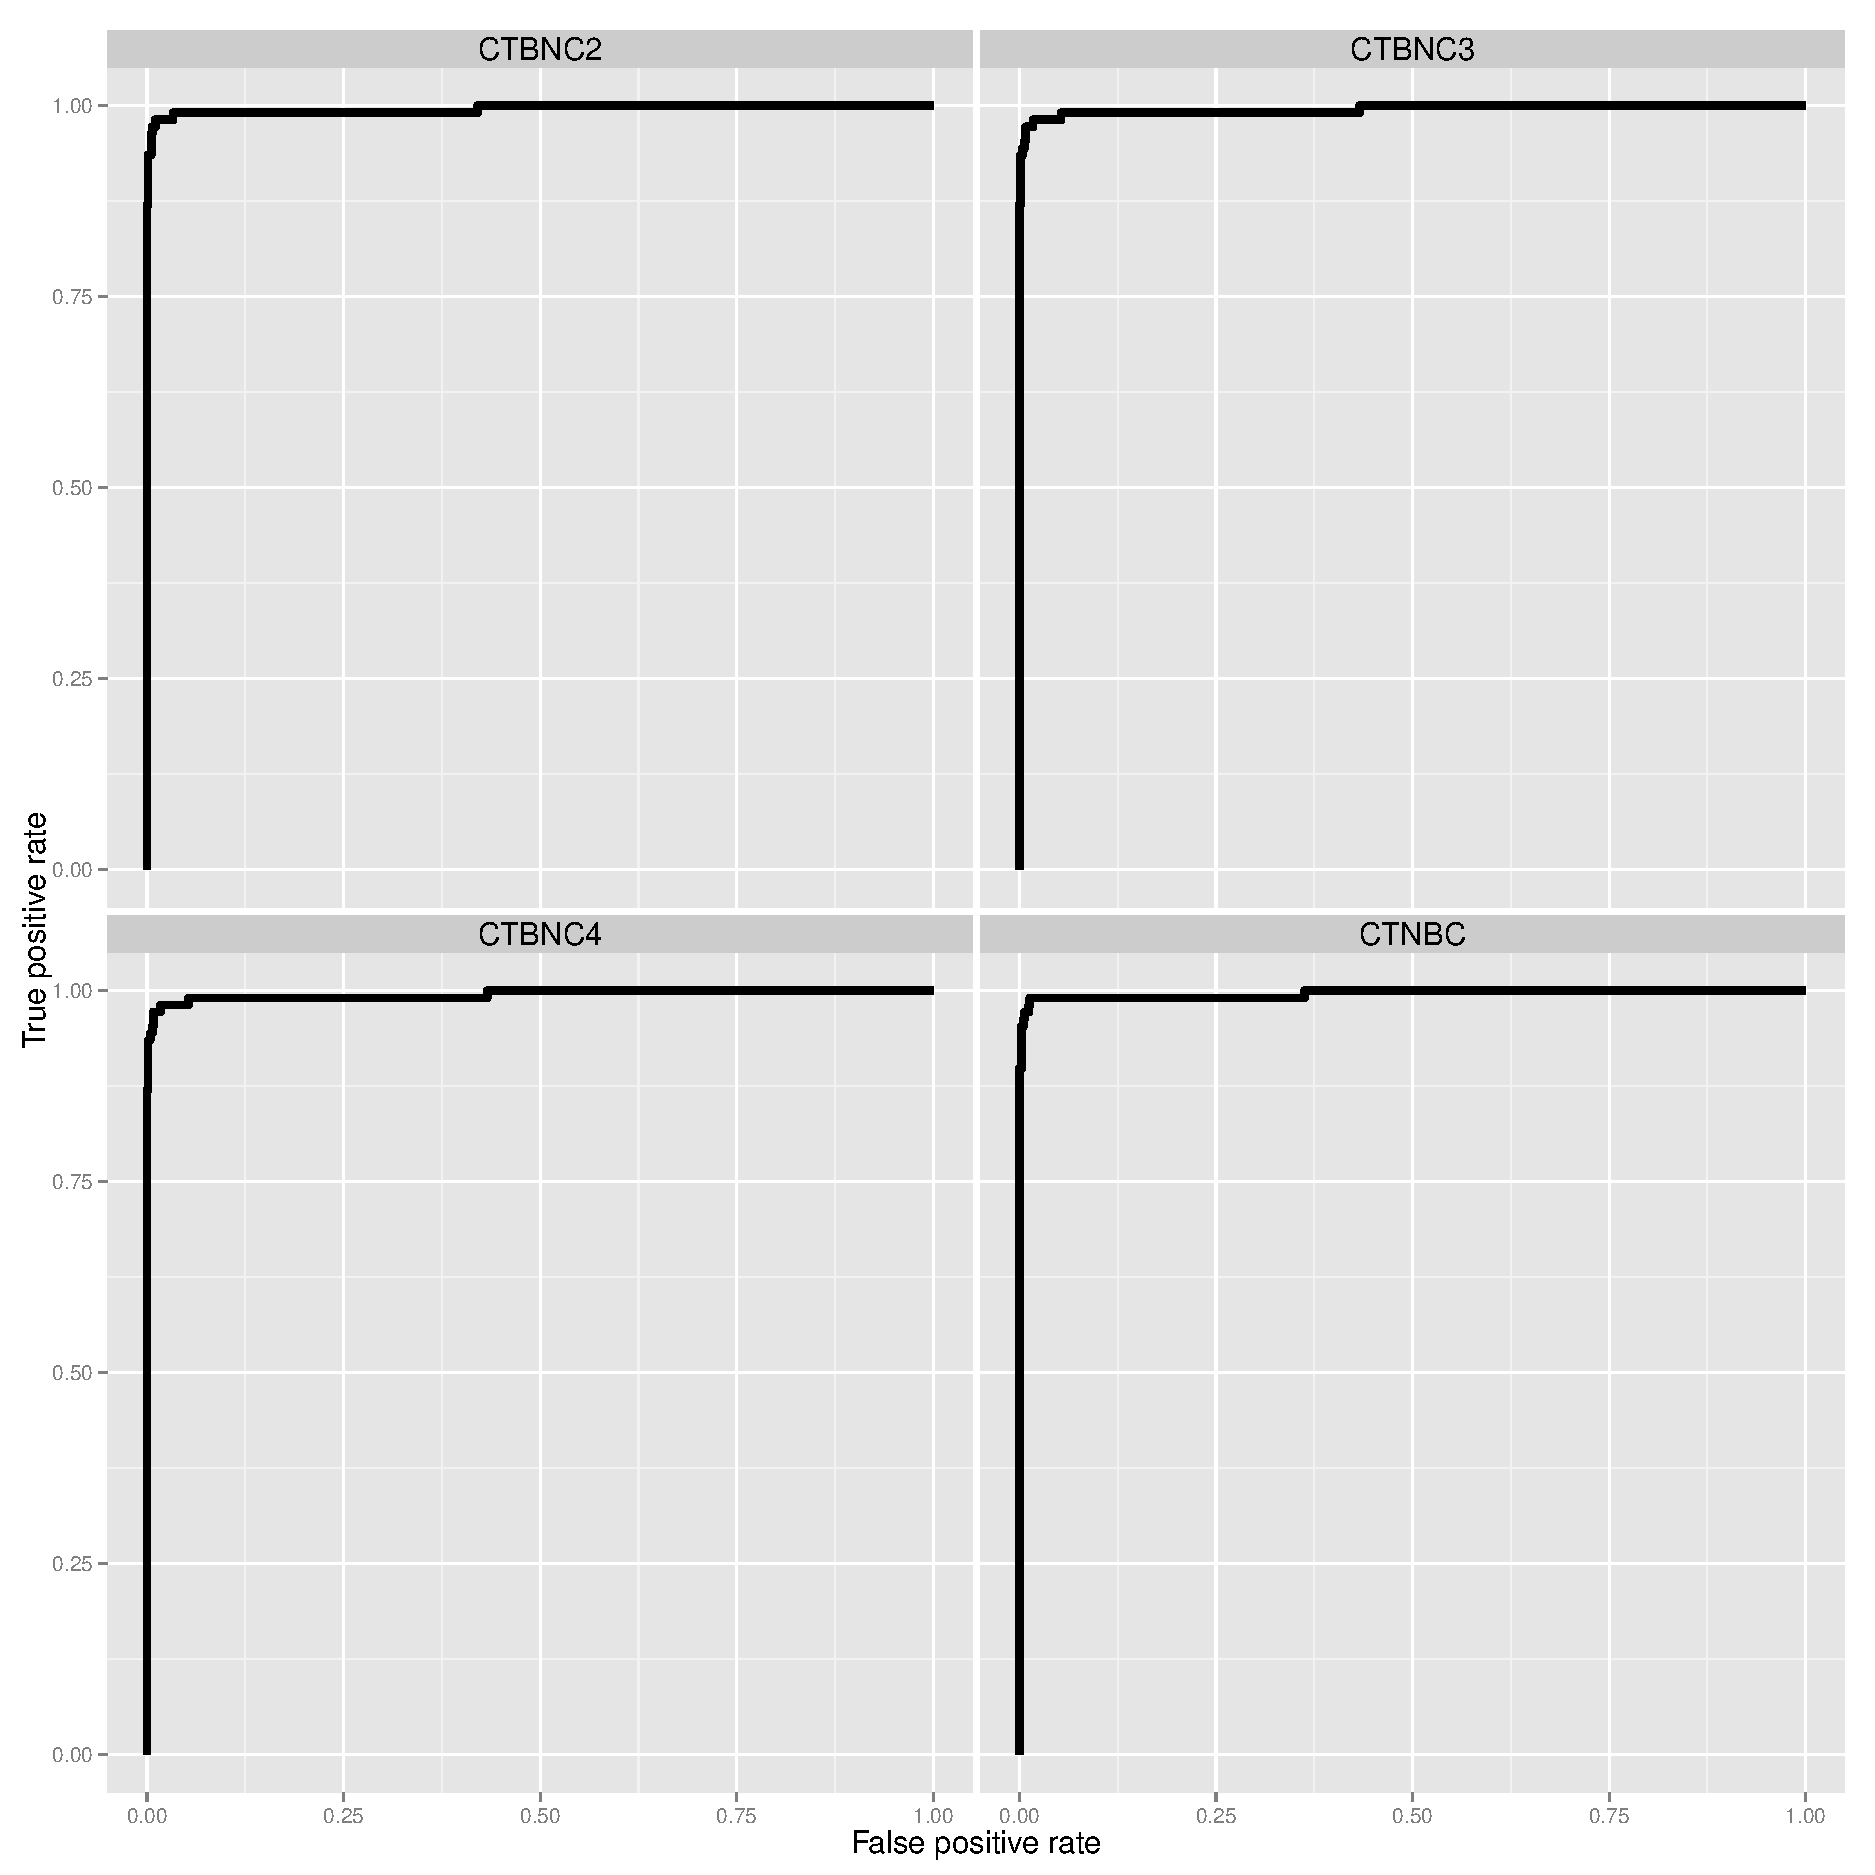
\includegraphics[width=1.05\textwidth,center]{microavg-model-rocs-class-01.pdf}
	\caption[Curve \acs{ROC} relative alla classe $1$]{Curve \acs{ROC}\index{risultati!\acsfont{ROC}}, relative alla classe $1$, di ogni classificatore utilizzato nel processo di sperimentazione.}
	\label{fig:roc-curves-class-1}
\end{figure}

\begin{figure}
	\centering
	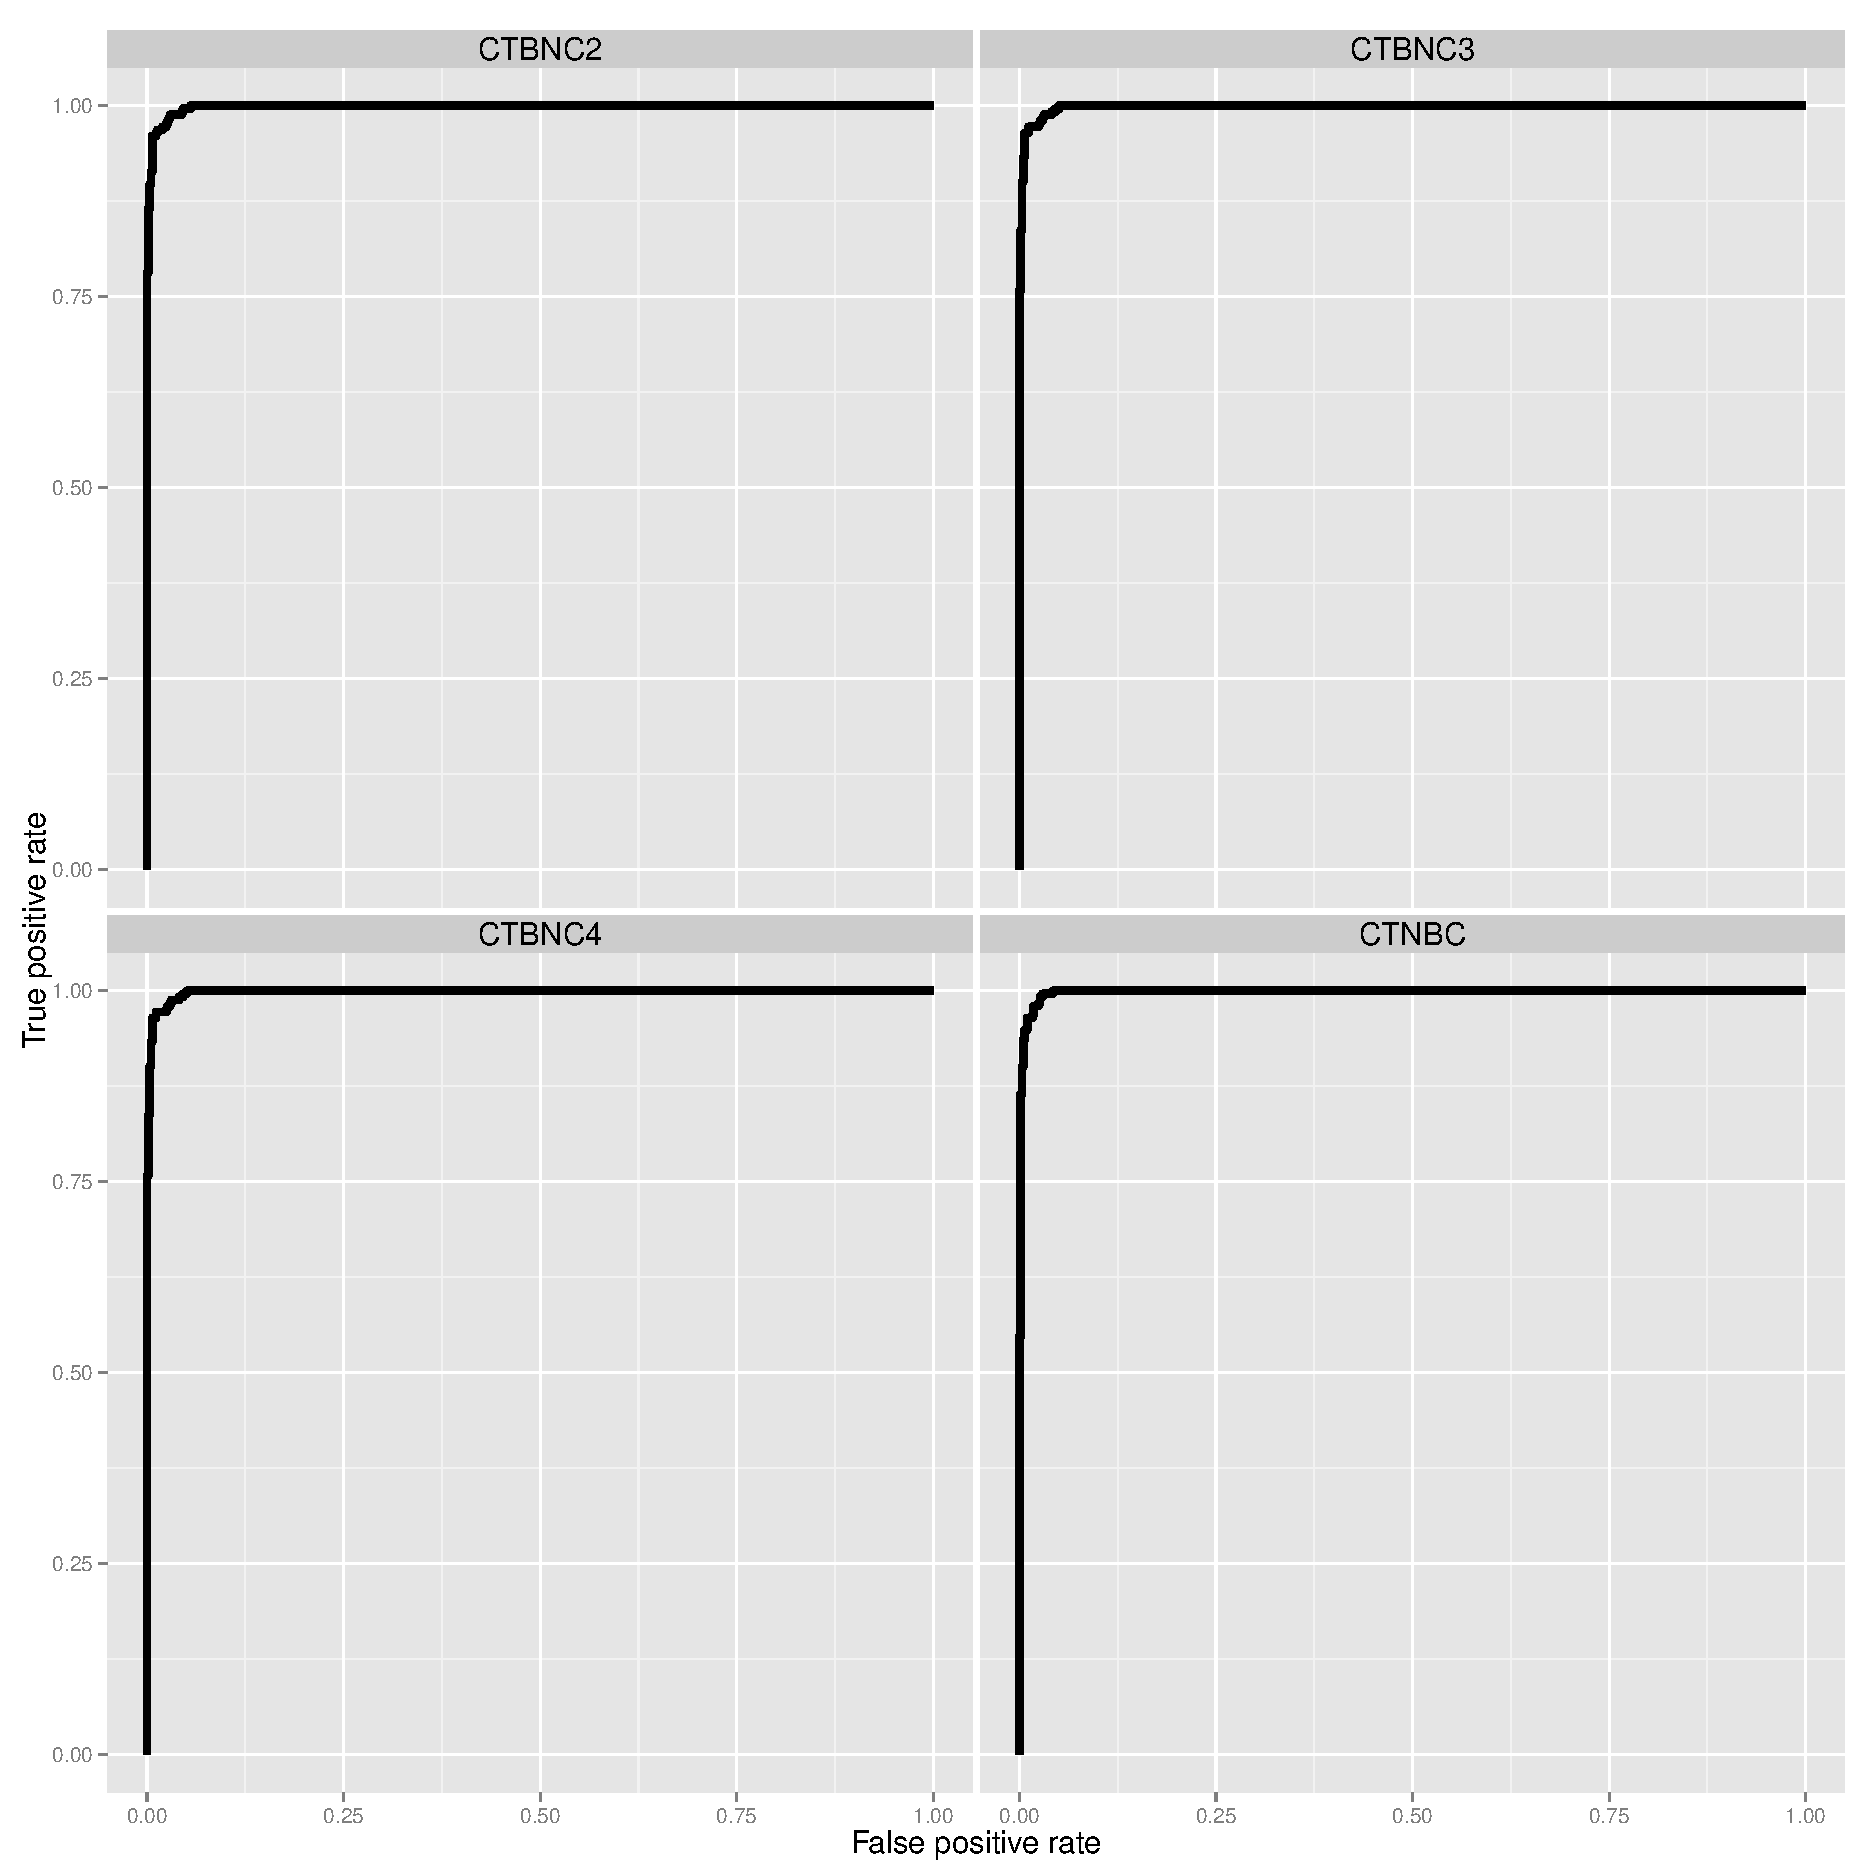
\includegraphics[width=1.05\textwidth,center]{microavg-model-rocs-class-02.pdf}
	\caption[Curve \acs{ROC} relative alla classe $2$]{Curve \acs{ROC}\index{risultati!\acsfont{ROC}}, relative alla classe $2$, di ogni classificatore utilizzato nel processo di sperimentazione.}
	\label{fig:roc-curves-class-2}
\end{figure}

\begin{figure}
	\centering
	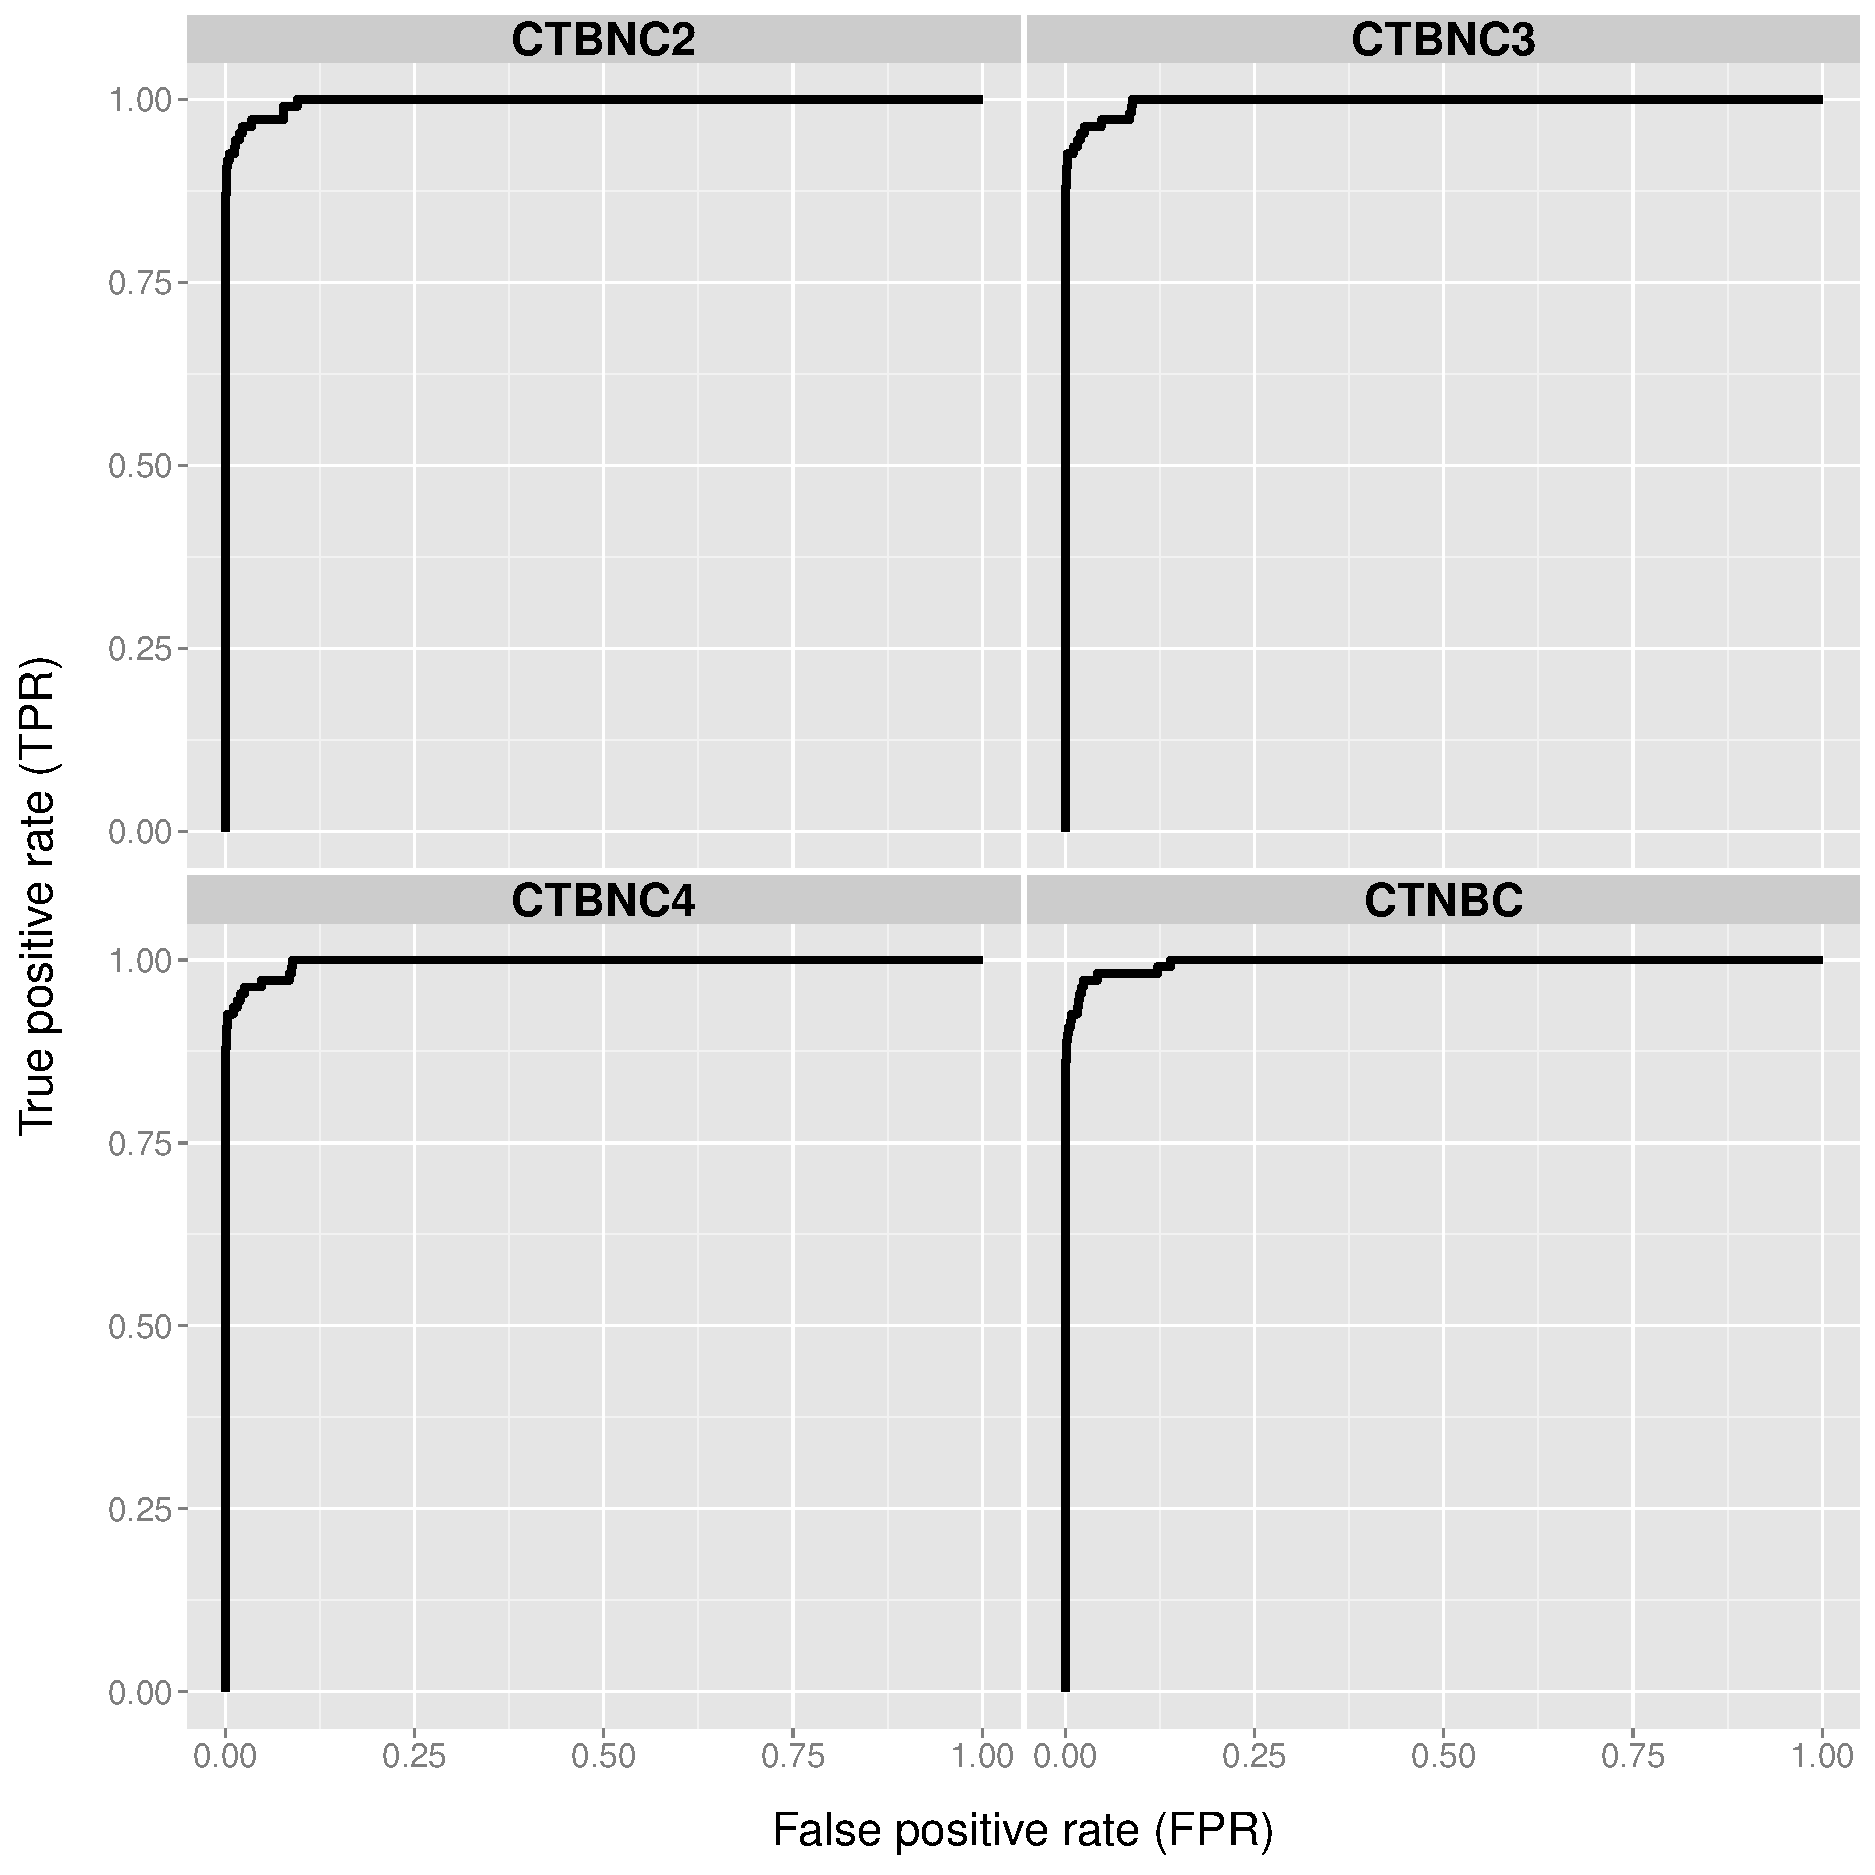
\includegraphics[width=1.05\textwidth,center]{microavg-model-rocs-class-03.pdf}
	\caption[Curve \acs{ROC} relative alla classe $3$]{Curve \acs{ROC}\index{risultati!\acsfont{ROC}}, relative alla classe $3$, di ogni classificatore utilizzato nel processo di sperimentazione.}
	\label{fig:roc-curves-class-3}
\end{figure}

\begin{figure}
	\centering
	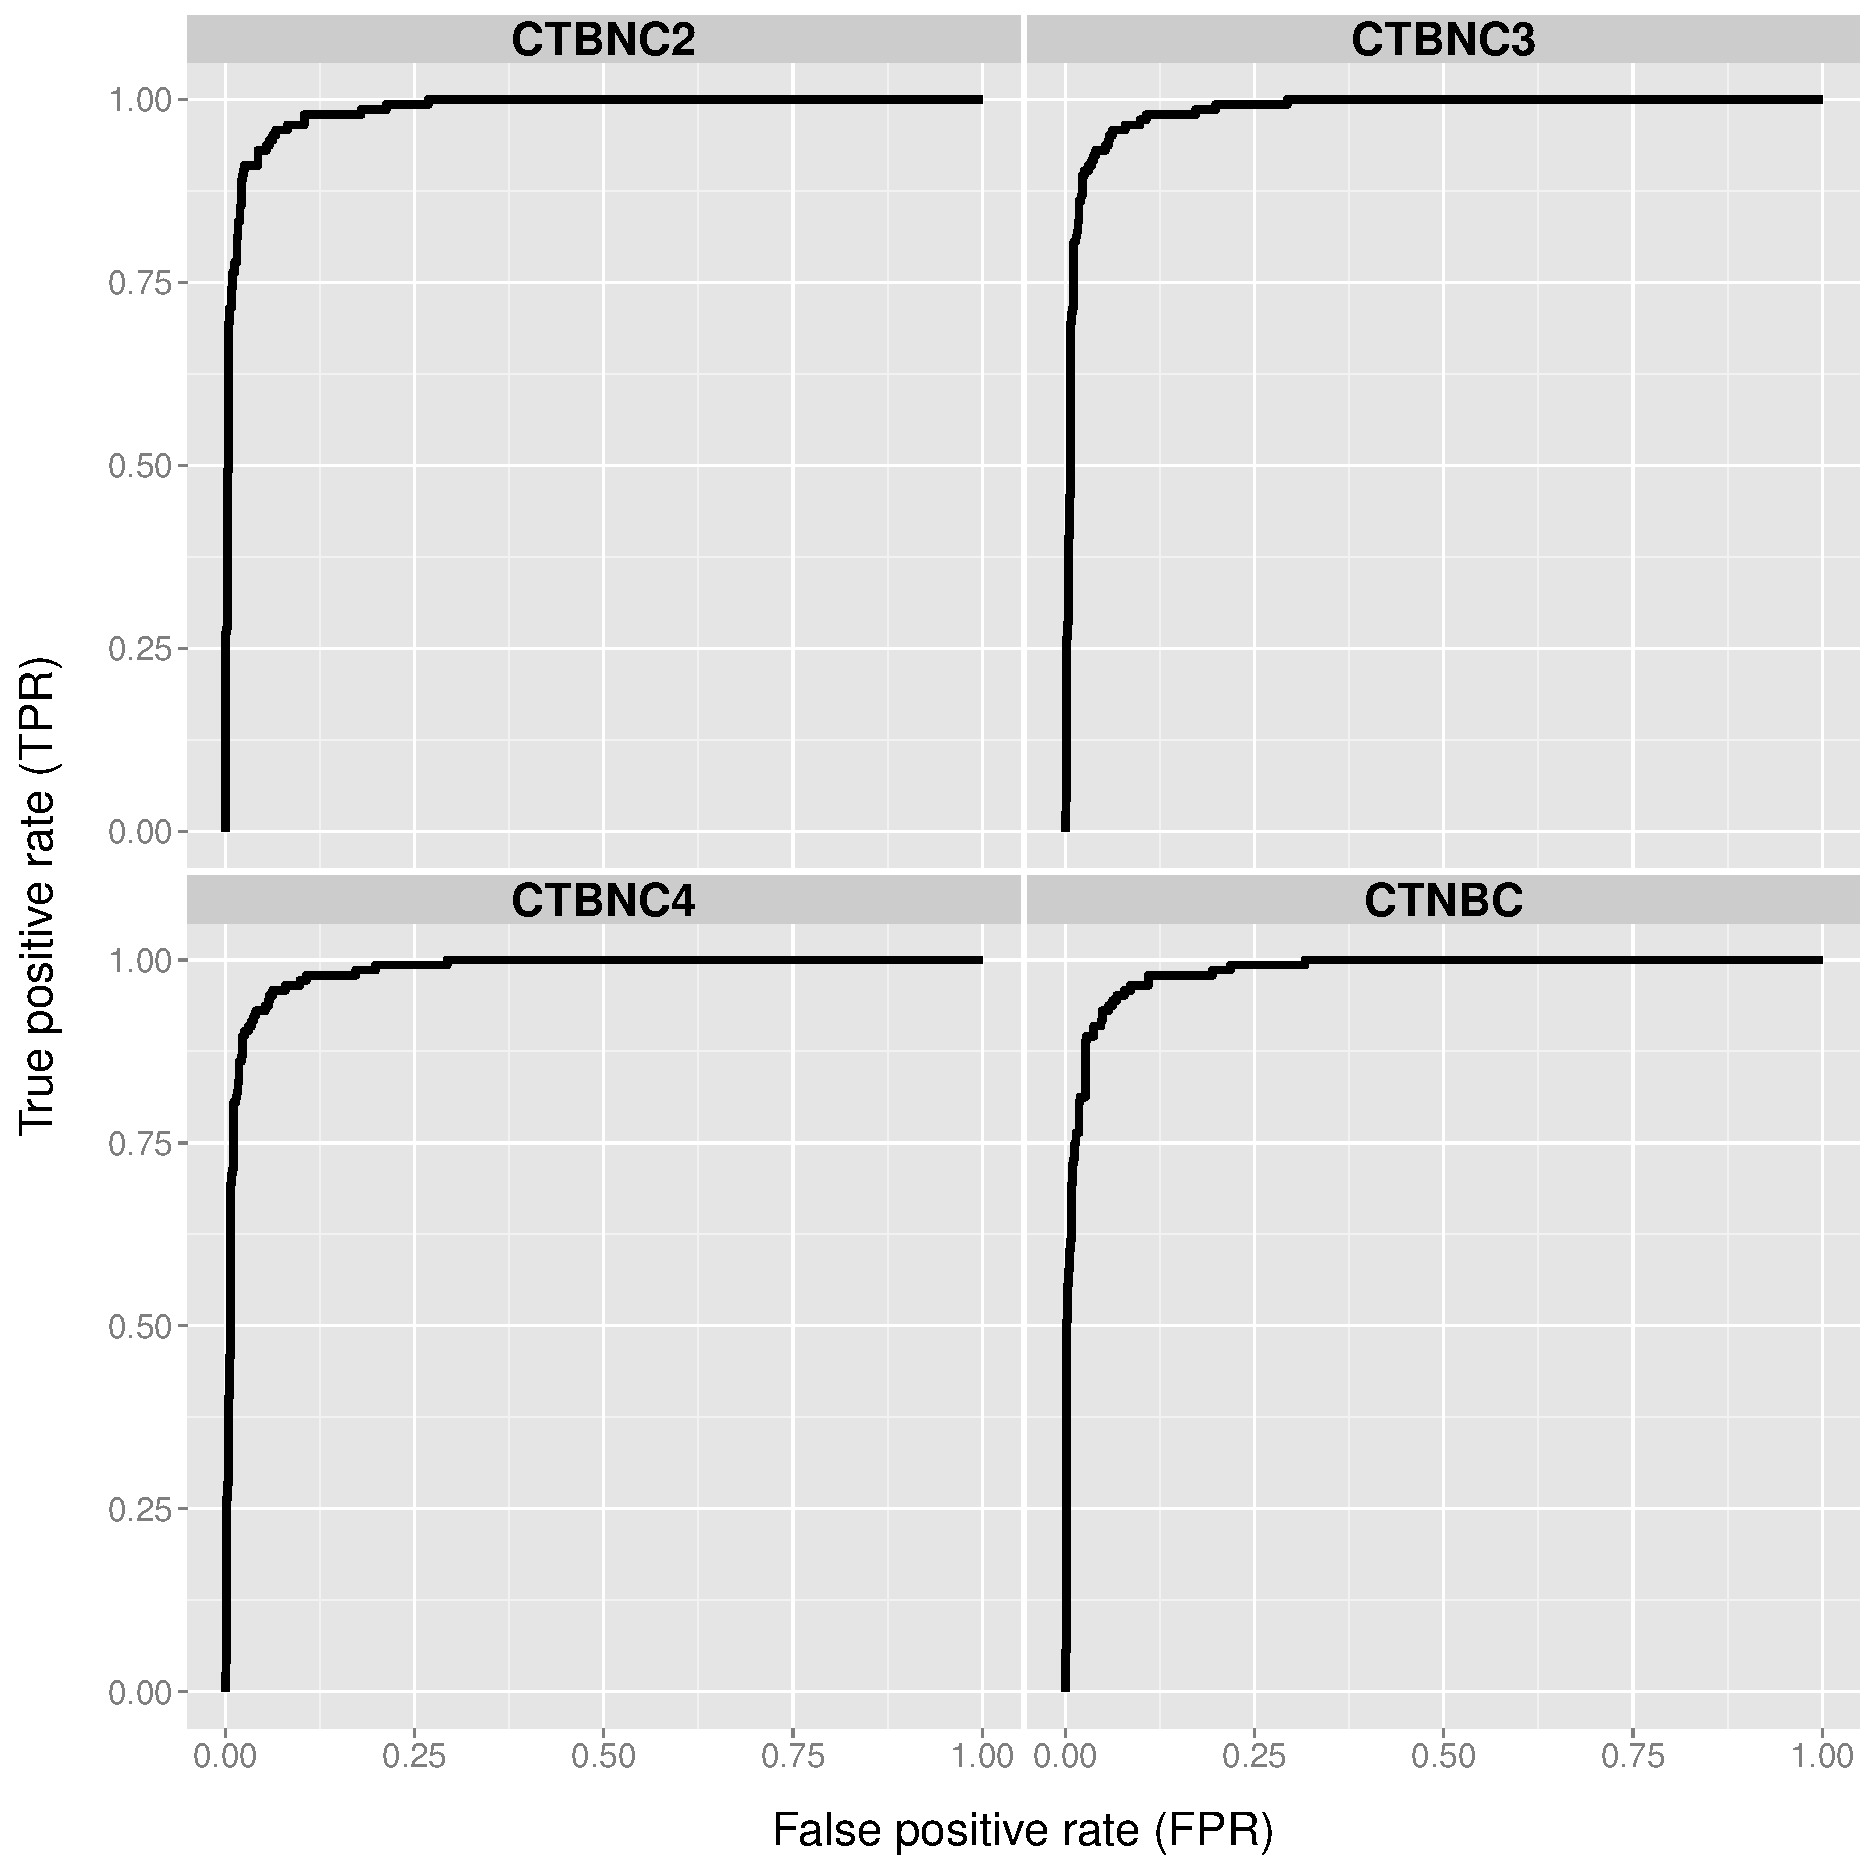
\includegraphics[width=1.05\textwidth,center]{microavg-model-rocs-class-04.pdf}
	\caption[Curve \acs{ROC} relative alla classe $4$]{Curve \acs{ROC}\index{risultati!\acsfont{ROC}}, relative alla classe $4$, di ogni classificatore utilizzato nel processo di sperimentazione.}
	\label{fig:roc-curves-class-4}
\end{figure}

\begin{figure}
	\centering
	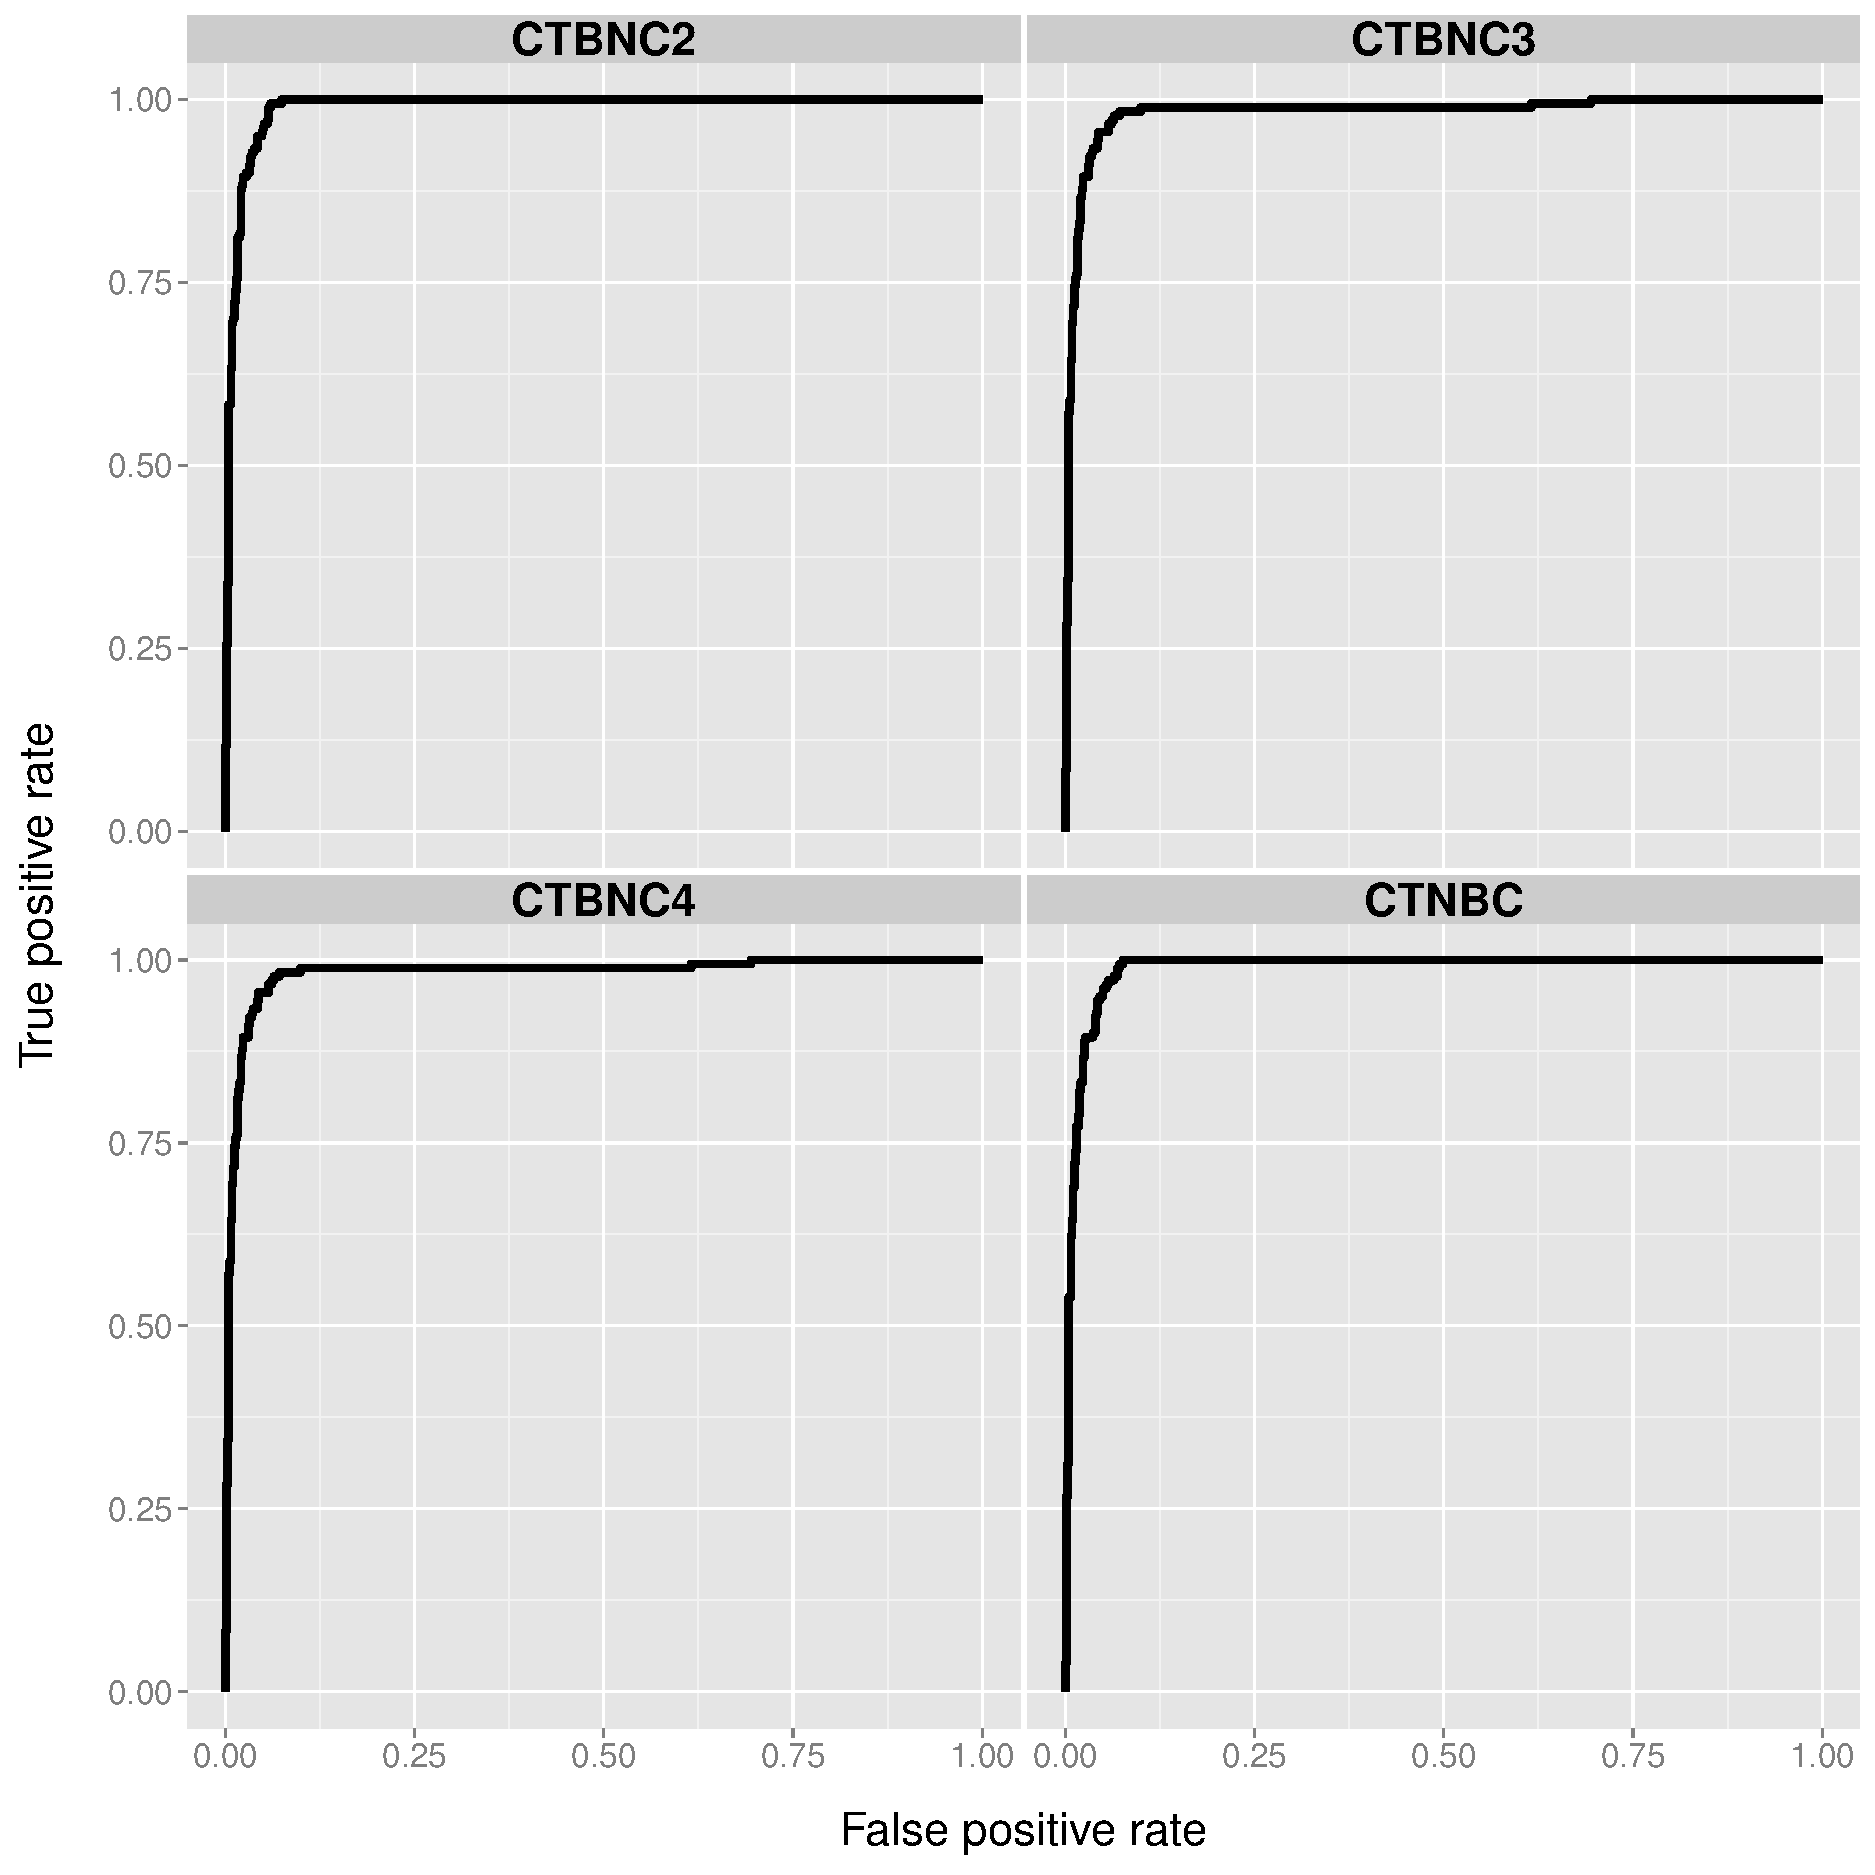
\includegraphics[width=1.05\textwidth,center]{microavg-model-rocs-class-05.pdf}
	\caption[Curve \acs{ROC} relative alla classe $5$]{Curve \acs{ROC}\index{risultati!\acsfont{ROC}}, relative alla classe $5$, di ogni classificatore utilizzato nel processo di sperimentazione.}
	\label{fig:roc-curves-class-5}
\end{figure}

\begin{figure}
	\centering
	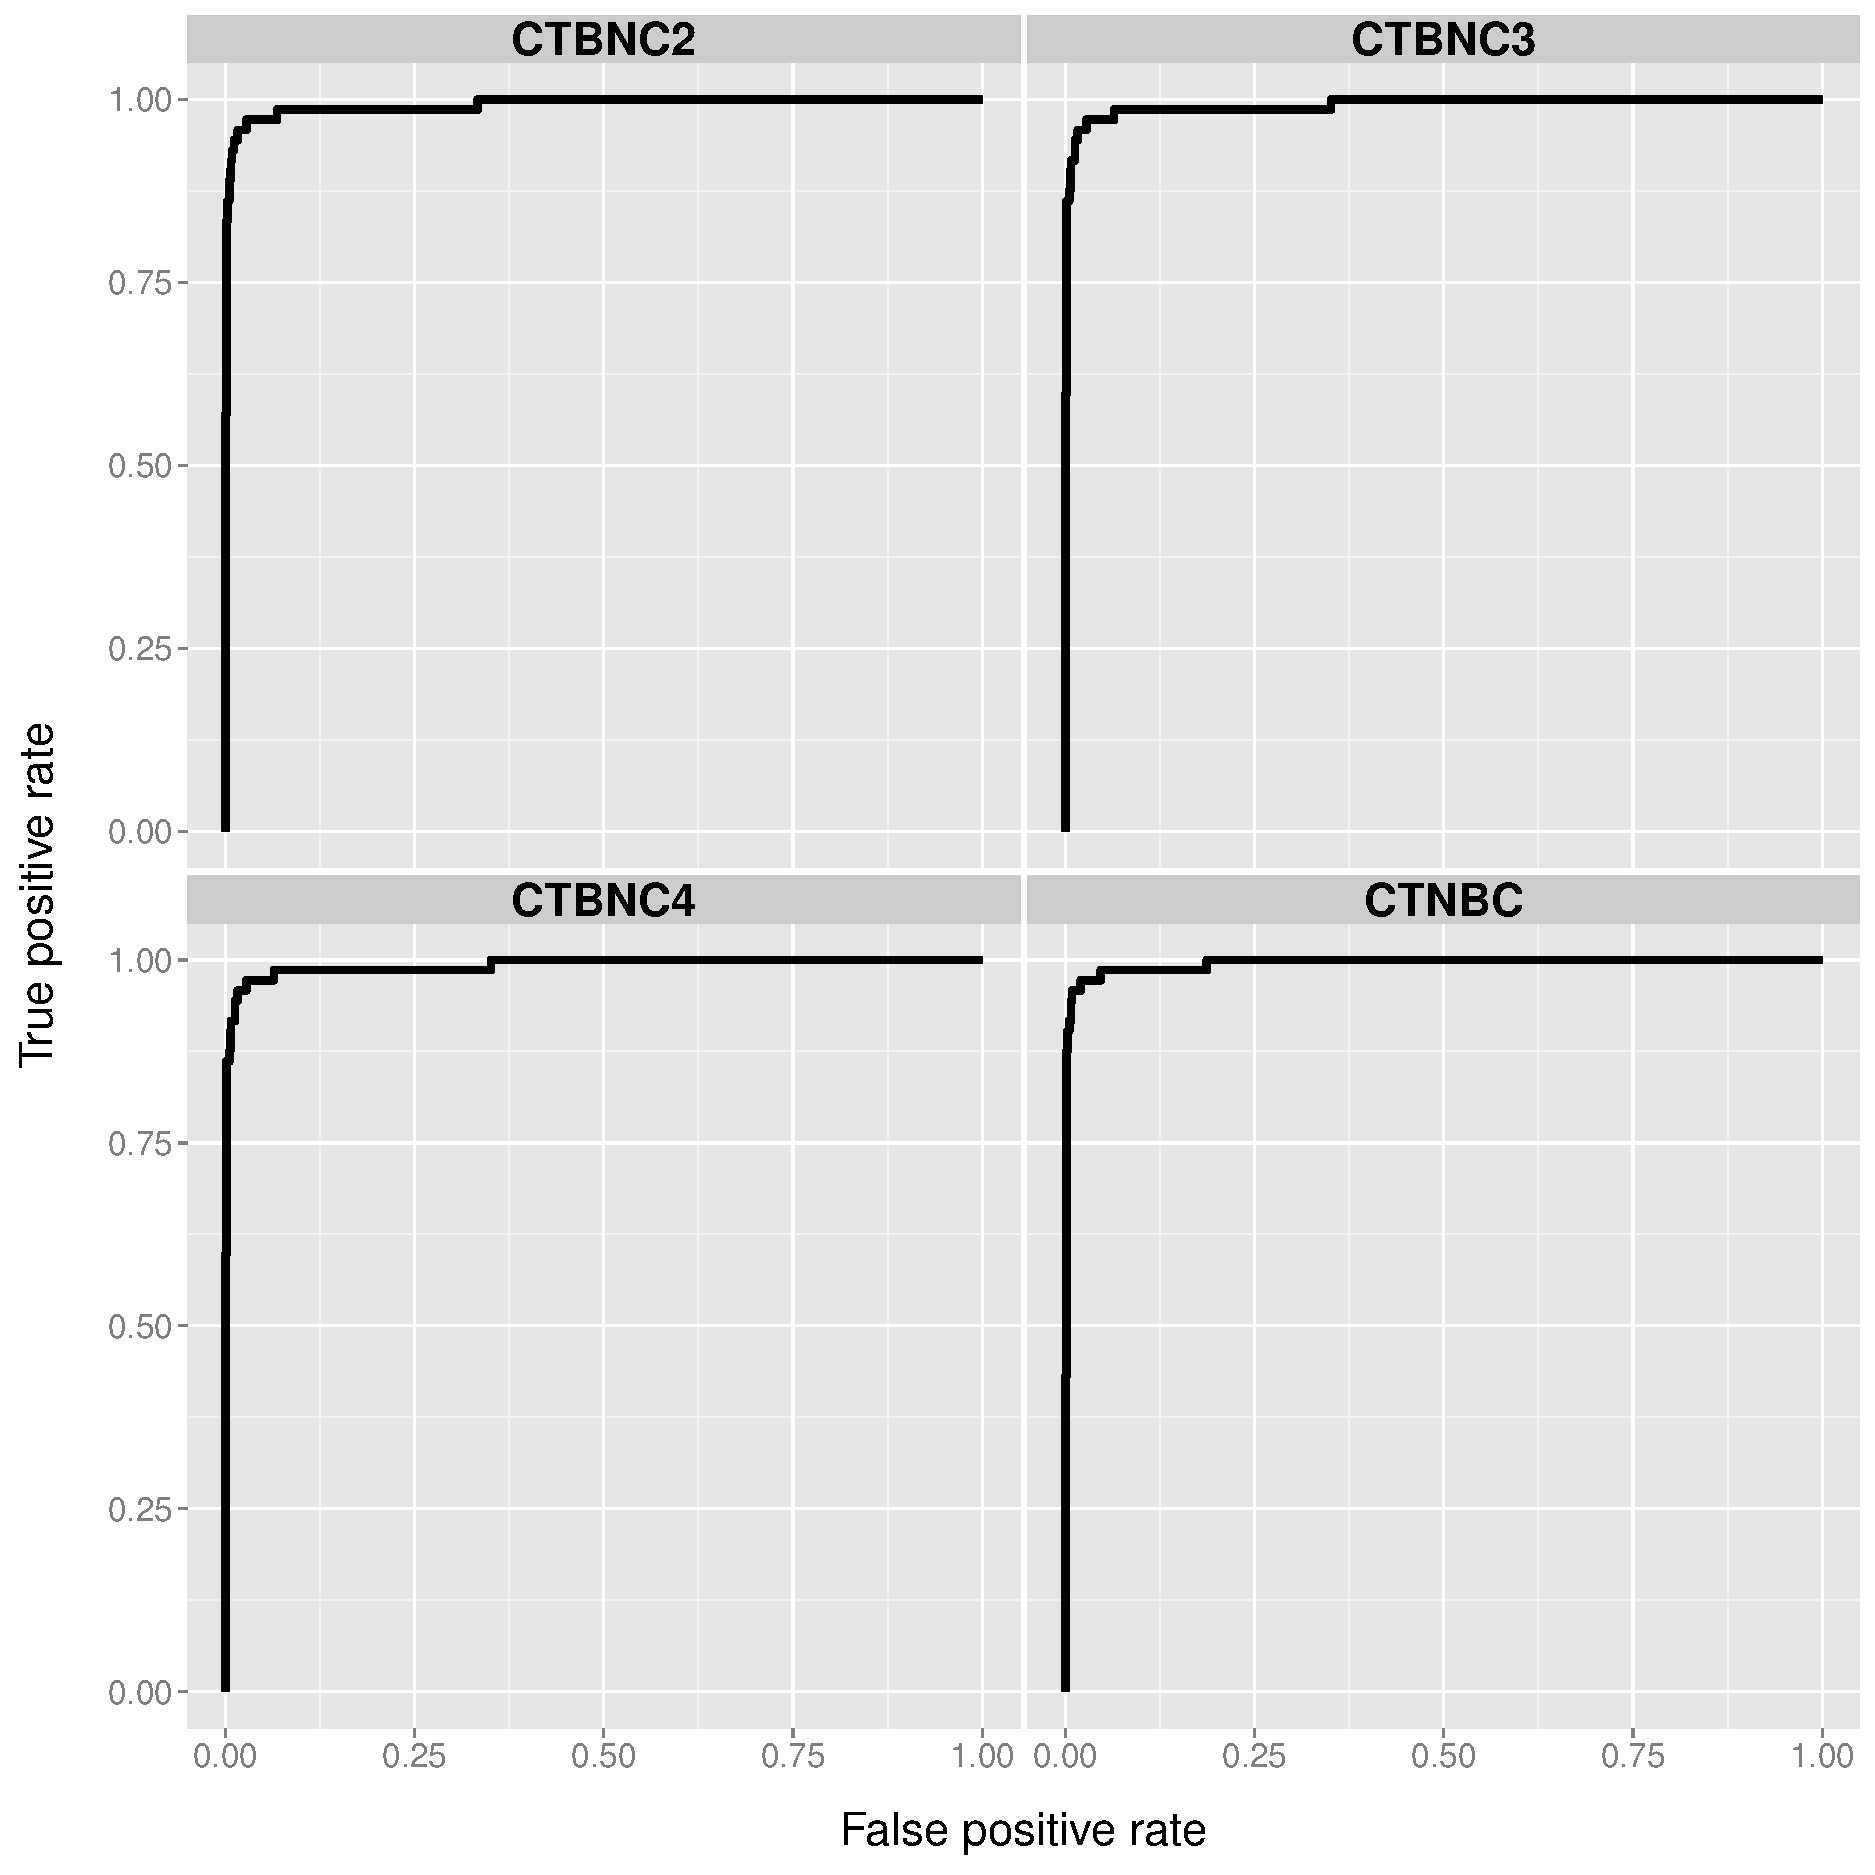
\includegraphics[width=1.05\columnwidth,center]{microavg-model-rocs-class-06.pdf}
	\caption[Curve \acs{ROC} relative alla classe $6$]{Curve \acs{ROC}\index{risultati!\acsfont{ROC}}, relative alla classe $6$, di ogni classificatore utilizzato nel processo di sperimentazione.}
	\label{fig:roc-curves-class-6}
\end{figure}
